\section{簡介}
%文獻上已經提出許多改進資料不足語言的句法剖析的方法,其中多半需要該資料不足語言的特性,用以找尋與其相似的語言進行協同訓練。
%近年來初見於影像領域的模型無關元學習,本來是為了處理少量樣本學習的問題,
%不久後也為資料不足(但資料量大於少量樣本學習)的學習任務所用\cite{gu-etal-2018-meta},
%不需要事先知道任務的特性,

\iffalse
有名的語言學家杭氏(Noam Chomsky)觀察人類習得語言的過程,
他認為嬰孩學習語言時所接收到的語言輸入是不足以讓他們習得該語言的所有特徵的,
許多特性相異的語法都可以產生這些他們所接收到的語料,
但孩童仍然習得了該語言的正確語法,
因此他推斷人類出生時大腦中即具備有某種語言習得裝置(Language acquisition device),
而語言習得裝置的任務便是從所有與語料匹配的語法中挑選正確的語法
\fi
本章介紹使用模型無關元學習進行多語言預訓練,以幫助資料不足語言的依存句法剖析的系列實驗。

模型無關元學習本來是為了處理圖片分類領域少量樣本學習的問題,
不久後也為資料不足(但資料量大於少量樣本學習)的學習任務所用,
如古氏(Jiatao Gu)將元學習方法引入資料不足的機器翻譯,
並勝過使用普通多語言學習的基準模型\cite{gu-etal-2018-meta}。
芬氏(Chelsea Finn)在2018年提出的模型無關元學習(model-agnostic meta-learning)
\cite{Finn2017ModelAgnosticMF}為所有使用梯度下降法(gradient descent)進行最佳化的模型提供了一項簡潔且有效的方法處理資料不足任務。
在語言轉移學習的框架下,其目標是替未見過的語言(unseen languages)尋找一合適參數初始值,使得少量步數梯度更新後,參數在該語言的測試集上表現最佳,
其稱此在少量步數更新就能大幅增進爲見過語言表現的能力為「快速適應」(fast adaptation)\cite{Finn2017ModelAgnosticMF}。
%其強調使用少量步數進行梯度更新,即是由於資料不足語言資料稀少,過多步數容易過擬合。

在元學習出現以前,
若希望利用相似語言中所蘊含的資訊給予模型語言普遍具備的歸納偏置(下稱普適語言偏置,universal linguistic biases),
多語言學習(multilingual learning)為一主要的方法\cite{caruana1997multitask}。
藉由共享特徵抽取網路並用以同時訓練多種相關語言,
相關語言的資訊得以透過反向傳播(backpropagation)注入類神經網路中,
使模型相較於解釋單一語言,更加偏好能夠解釋所有相關語言的假說,
有效幫助模型達成泛化(generalization)。

然而多語言訓練的目標,是提高訓練語言(training languages)在其測試集(testing set)上的準確率,
而提高訓練語言的準確率,未必就代表在資料不足語言上的準確率也會隨之提高;
有可能出現訓練語言與資料不足語言差異過大,而導致多語言訓練模型無法幫助資料不足語言的任務表現。

不若單純的多語言訓練,模型無關元學習於訓練階段的目標並非提高在訓練語言上的表現,
而是直接最佳化模型在未見過語言上\finetune 後的表現,訓練與測試環境沒有不匹配之處,
有效防止模型只在訓練語言的測試集上有好表現,而無法推廣到資料不足語言上的問題。

\iffalse
尤其當目標任務缺乏資料的時候,若使用過於有表現力的假說集合,
易使模型過擬合到目標任務上,
利用相似任務進行多工學習幫助目標任務提升表現的效果尤其顯著。
然而多工學習得到的模型可以在訓練過的所有任務上的測試集有好表現,
但並未保證這樣的好表現可以轉移到相似但未見過的任務上;
而芬氏(Chelsea Finn)提出的模型無關元學習(model-agnostic meta-learning)
\cite{Finn2017ModelAgnosticMF}提供了多工學習之外的另一種方法,
將領域的歸納偏置(inductive bias)注入類神經網路中。
\fi

%\section{相關研究}


\section{多語言去詞化依存句法分析(multilingual delexicalized dependency parsing)}
由於詞化的依存句法分析有太多變因,包括使用的預訓練模型,其對不同語言的偏置等等,都會影響句法剖析模型於目標語言上的行為;
且詞化的依存句法分析參數量較多,使用二次微分的計算量與佔用空間均較大,訓練耗時,
有時甚至會發生用來進行平行矩陣運算的圖形處理器記憶體不足的問題。
因此為了排除語言本身句法以外性質對句法剖析的影響及計算資源的考量,
本節先進行去詞化依存句法分析的實驗,
也就是只使用句法樹庫提供的詞性標記做為詞的表徵進行句法剖析。

\subsection{詞性標記(POS tags)}
UD句法樹庫中大部分的語言均提供兩種詞性標記:專為該語言設計的詞性標記(XPOS),通常為該句法樹庫尚未整合進UD時原本的詞性標記,
與各語言統一的普適詞性標記\cite{petrov-etal-2012-universal}(Universal POS tags, UPOS),
其捨棄各語言細緻的詞性分別,
整合語言間相似性質的詞性,以達到所有語言共享同一組詞性集合的目標。
如前置介系詞(prepositions)與後置介系詞(postpositions)在UPOS的框架下就被整合成介系詞(adpositions)而不做前後置之分。
由於UPOS有更好的跨語言通用性,本研究去詞化句法剖析的詞性標記輸入均使用UPOS。

\subsection{修訂版爬蟲類元學習}
原始版本的爬蟲類元學習\cite{nichol2018first}無論是在內循環或外循環的開頭都不會重新啟動內循環的優化器,
當使用有動能(momentum)的優化器如Adam時,當下的梯度更新會受之前用其他語言計算而得的梯度影響,
造成語言間不必要的干擾。
為了避免此現象,原作者將一階動能項$\beta_{1}$設為$0$。
%然而mBERT原始論文中進行精細校正使用的為具有動能項的Adam,
然而本研究的初始實驗發現$\beta_{1} = 0$的Adam在精細校正時時會對準確率造成負面影響。
再者,爬蟲類元學習將外循環原始梯度(raw gradient)直接設為各語言內循環(亦即精細校正)前後參數的差異的平均,
此數值大小很大程度上取決於內循環優化器的學習率,
恐與一般模型精細校正時接收到的梯度分佈差異過大。

為處理此問題,本研究稍稍修改了爬蟲類元學習的演算法,
希望在不改變內循環優化器設置的前提下保留爬蟲類元學習加總內循環所有梯度的優點:
與其將內循環梯度設為前後參數的差異的平均 $\phi - U_{\textrm{ADAM}}^{k}(\phi) $,
內循環原始梯度經過內循環優化器處理過後的產物,
本研究將內循環梯度直接設為內循環\textbf{原始}梯度的平均(此處優化器以Adam為例):
\begin{equation}
    g_{\textrm{REP}} = \mathbb{E}_{\tau}\left[ \frac{1}{k} \sum_{i=1}^{k} \nabla_{\phi_{i}} \mathcal{L}_{\tau} \left( \phi_{i}^{\texttt{adam}} \right) \right]
\end{equation}
其中
\begin{equation}
    \phi_{i}^{\texttt{adam}} = U_{\textrm{ADAM}} \left( \phi_{i - 1}^{\texttt{adam}} \right).
\end{equation}
此數值雖然是由內循環優化器計算出來,但此處取其原始梯度,
受內循環學習率影響較小。
此修訂版爬蟲類元學習與普通的多語言學習的差異比起原始的爬蟲類元學習要來的更小:
外循環的梯度為內循環原始梯度的平均,與多語言學習類似;
但原始梯度仍是由內循環更新過的參數計算出來的(除了內循環的第一步),更接近原本的爬蟲類元學習。
初始實驗發現此修訂版爬蟲類元學習表現不俗,
且相較原始爬蟲類元學習的表現來的更加穩定。
往後提到的爬蟲類元學習均意指本節所提出的修訂版爬蟲類元學習。

\subsection{實驗設置}
\label{subsec:delex_depparse_setting}

\begin{table}[htbp]
    % \fontsize{8}{10}\selectfont
    \centering
    \begin{subtable}[t]{.4\textwidth}
        \begin{tabular}[t]{@{}lr@{}}
        \toprule
        超參數 & 值 \\
        \midrule
            詞性嵌入維度         & 100 \\
            編碼器              & 雙向LSTM \\
            編碼器層數           & 3 \\
            編碼器隱維度         & 100 \\
            依存標籤維度         & 200 \\
            依存邊維度           & 200 \\
            詞性丟棄機率            & 0.33 \\
            批次大小$b$         & 16 \\
            語言數$l$           & 10 \\
            訓練樣本數/回合        & 64000 \\
            訓練回合數          & 10 \\
            優化器              & Adam \\
            $\beta_1,\beta_2$  & 0.9, 0.9 \\
            權重衰減參數         & 0.01 \\
            基礎學習率          & $3e^{-4}$ \\
            最大梯度範數        & 5.0 \\
        \bottomrule
        \end{tabular}
        \caption{
            預訓練超參數。
        }
        \label{tab:delex_pretrain_hparams}
    \end{subtable}
    \begin{subtable}[t]{.4\textwidth}
        \begin{tabular}[t]{@{}lr@{}}
        \toprule
        超參數 & 值 \\
        \midrule
            優化器              & Adam \\
            基礎學習率          & $3e^{-4}$ \\
            $\beta_1,\beta_2$  & 0.9, 0.9 \\
            批次大小            & 16 \\
            訓練回合數          & 80 \\
            最大梯度範數        & 5.0 \\
            交叉驗證摺數$k$     & 3   \\
        \bottomrule
        \end{tabular}
        \caption{
            精細校正超參數。
        }
        \label{tab:delex_finetune_hparams}
    \end{subtable}
    \caption{
        模型超參數一覽。
    }
    \label{tab:delex_hparams}
\end{table}
我們從\conll 的53種訓練語言(73個訓練句法樹庫)中選取有官方驗證集(development set)的46種訓練語言(66個訓練句法樹庫)作爲訓練語言;見表\ref{tab:training_languages}。
預訓練完成後,我們分別對該模型進行\zeroshot 及\finetune 在預訓練中未見過的語言上。
我們挑選\conll 的訓練語言中剩下的只有訓練集而沒有發展集的語言作爲真實資料不足測試語言(true low-resource testing languages,見表\ref{tab:true_lr_testing_languages})。
為了觀察控制資料多寡時對不同預訓練方法的影響,
我們另外挑選了UD 2.5版中8種不在訓練語言中的語言做為模擬資料不足測試語言(simulated low-resource testing languages,見表\ref{tab:sim_lr_testing_languages})。
實驗在訓練與測試時時均使用正確的斷句、斷詞,並使用句法樹庫提供的正確詞性做為詞的表徵。

至於多語言訓練的部分,孔氏\cite{kondratyuk-straka-2019-75}與烏氏\cite{ustun2020udapter}進行多語言訓練的方法,
是將全部語言的句法樹庫接在一起、在一個小批次(batch)中混合多個句法樹庫訓練。
這樣的做法可能會導致資料量大的語言取樣頻率過高;
我們的方法則是每次更新從全部語言裡取樣$l$種語言,每種語言取樣$b$個句子,一個批次總共有$b \times l$個句子。
不同於孔氏與烏氏,這樣的方法防止模型過度對資料充足語言的特性建模,但也可能使得資料不足語言的句子被過度取樣而產生過擬合的現象。

超參數的設置見表\ref{tab:delex_hparams}。
\subsection{實驗結果}

\begin{figure}[htbp]
    \centering
    \begin{subfigure}[t]{\textwidth}
        \centering
        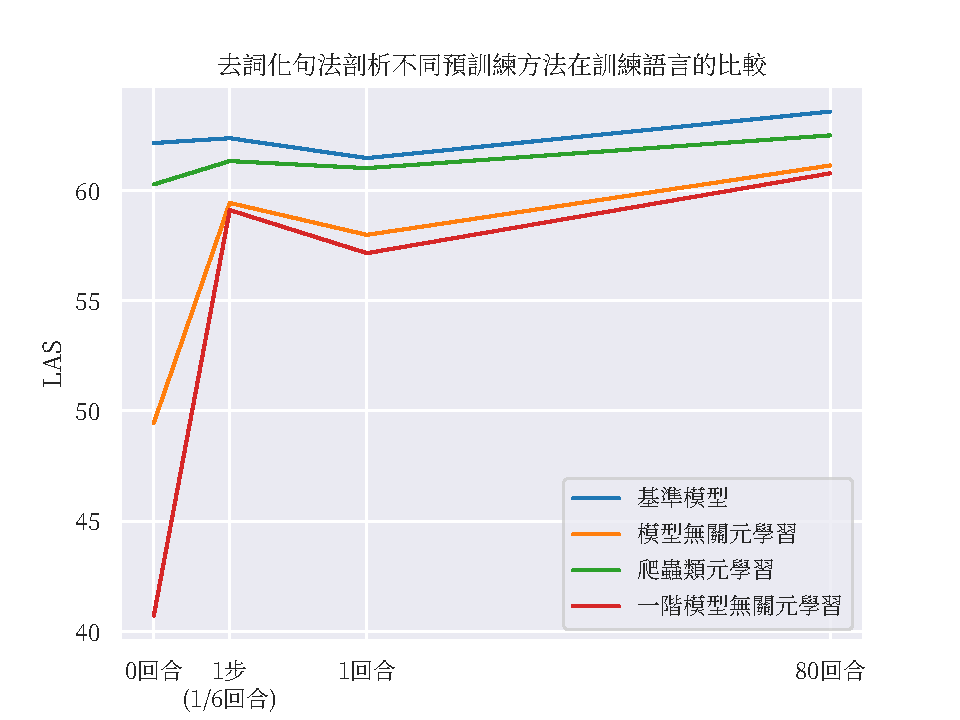
\includegraphics[width=\textwidth]{figs/chapter3/delex/delex_train_langs.pdf}
    \end{subfigure}
    \vspace{-12pt}
    \begin{subfigure}[t]{\textwidth}
        \centering
        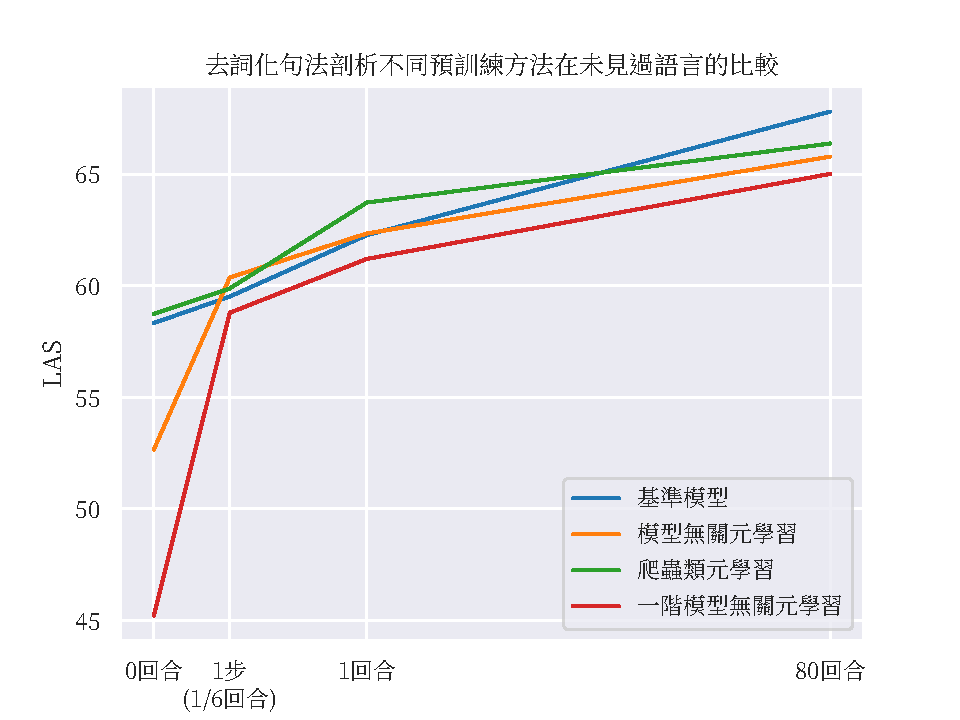
\includegraphics[width=\textwidth]{figs/chapter3/delex/delex_test_langs.pdf}
    \end{subfigure}
    \caption{去詞化分析不同預訓練方法精細校正後在測試集上的平均表現。}
    \label{fig:delex_avg}
\end{figure}
圖\ref{fig:delex_avg}為去詞化分析不同預訓練方法產生的模型在目標語言上經過不同步數的\finetune 後的測試集LAS數值。
由圖中可以觀察到:
\begin{itemize}
    \item 在未見過語言上,模型無關元學習模型於只精細校正一步的表現及相對於精細校正前的進步量均為各方法中之冠,
顯示模型無關元學習的確有快速適應的能力。
    %\item 在未見過語言上,模型無關元學習於
    \item 模型無關元學習模型在零樣本學習的表現大幅落後基準模型,說明其優勢主要在只需少量目標語言資料即可快速適應的能力,
    並不適合做為單一多語言模型同時處理多種語言。
    \item 在未見過語言上,\reptile 模型在零樣本學習、精細校正一步、一回合與八十回合的情況下表現均與基準模型不相上下,
在精細校正一步與一回合更稍稍勝過基準模型,顯示其適合用於剖析所有訓練與未見過的語言,又能夠受益於少量未見過語言的語料。
    \item 在所有語言上,無論接觸多少目標語言的語料(精細校正前、一步、一回合、八十回合),
\fomaml 模型均大幅落後其他所有模型,顯示只取內循環最後一步的梯度更新既不足以使模型學習到訓練語言的語法,
也無法泛化到未見過的語言上。
    \item 在訓練語言上,基準模型無論接觸多少目標語言的資料,其表現均大幅贏過模型無關元學習模型,
這說明基準模型的確達到其訓練目標-同時剖析所有的訓練語言。

    %\item 在訓練語言上在精細校正一步的設置中,模型無關元學習模型在訓練語言上以少量資料精細校正後,於測試集上的表現明顯不如基準模型,但在未見過語言以少量資料精細校正測試集上
\end{itemize}

以下為分語言、分接觸目標語言語料量的數據圖表。
%其中表\ref{tab:delex_las_epoch_1}
其中圖\ref{fig:bar_zs}、\ref{fig:bar_one_step}、\ref{fig:bar_full_epoch_1}、\ref{fig:bar_full_epoch_80}
為各方法接觸不同數量的各種目標語言的語料其表現的長條圖。
\iffalse
\begin{table}[htbp]
    \begin{subtable}[h]{0.8\textwidth}
        \centering
            \begin{tabular}[!ht]{c|llll}
                \hline
                語言 & 基準 & 模型無關元學習 & 爬蟲類元學習 & 一階模型無關元學習 \\
                \hline\hline
                wo & \textbf{62.83}** & 55.47 & \textbf{62.96}** & 45.69 \\
                gd & \textbf{44.47} & 37.42 & \textbf{44.14} & 34.97 \\
                te & 60.61 & 60.06 & \textbf{62.55} & 52.15 \\
                cop & \textbf{66.58} & 63.17 & \textbf{66.93} & 59.33 \\
                be & \textbf{71.87}** & 57.70 & 70.78 & 45.26 \\
                mr & \textbf{48.30}* & 42.48 & \textbf{47.33}* & 34.22 \\
                mt & \textbf{68.76}** & 61.77 & \textbf{68.42}** & 57.40 \\
                ta & 43.19 & 43.19 & \textbf{46.81}** & 32.73 \\
                \hline
                avg & 58.33 & 52.66 & \textbf{58.74} & 45.22 \\
                \hline
            \end{tabular}
            \caption{未精細校正(0回合)。}
    \end{subtable}
    \vfill
    \begin{subtable}[h]{0.8\textwidth}
        \centering
            \begin{tabular}[!ht]{c|llll}
                \hline
                語言 & 基準 & 模型無關元學習 & 爬蟲類元學習 & 一階模型無關元學習 \\
                \hline\hline
                wo & 63.64 & 63.91 & 63.39 & \textbf{64.22} \\
                gd & 46.49 & 45.87 & \textbf{47.96}* & 46.88 \\
                te & 64.36 & 65.05 & \textbf{65.60} & 62.55 \\
                cop & 67.03 & 66.99 & \textbf{67.44} & 66.93 \\
                be & \textbf{71.59}** & 69.13 & \textbf{71.11}** & 67.99 \\
                mr & 48.79 & \textbf{53.40}** & 47.57 & 48.54 \\
                mt & \textbf{68.84}* & 68.08 & \textbf{68.83}* & 68.04 \\
                ta & 45.35 & \textbf{50.48}** & 47.11 & 45.15 \\
                \hline
                avg & 59.51 & \textbf{60.36} & 59.88 & 58.79 \\
                \hline
            \end{tabular}
        \caption{精細校正1步($\frac{1}{6}$回合)。}
    \end{subtable}
    \vfill
    \begin{subtable}[h]{0.8\textwidth}
    \centering
        \begin{tabular}[!ht]{c|llll}
            \hline
            語言 & 基準 & 模型無關元學習 & 爬蟲類元學習 & 一階模型無關元學習 \\
            \hline\hline
            wo & 65.71 & 63.43 & \textbf{66.53}* & 61.40 \\
            gd & 53.79 & \textbf{57.30}** & \textbf{57.11}** & 55.74 \\
            te & 68.24 & 67.27 & \textbf{70.18} & 64.77 \\
            cop & 66.95 & 65.83 & \textbf{67.84}** & 64.86 \\
            be & \textbf{69.14}** & 65.57 & \textbf{69.51}** & 65.96 \\
            mr & 52.67 & \textbf{58.25} & 55.10 & 56.55 \\
            mt & \textbf{70.05}** & 67.33 & 69.20 & 66.83 \\
            ta & 51.58 & 53.75 & \textbf{54.35} & 53.49 \\
            \hline
            avg & 62.27 & 62.34 & \textbf{63.73} & 61.20 \\
            \hline
        \end{tabular}
        \caption{精細校正1回合。}
    \end{subtable}
    \vfill
    \begin{subtable}[h]{0.8\textwidth}
        \centering
            \begin{tabular}[!ht]{c|llll}
                \hline
                語言 & 基準 & 模型無關元學習 & 爬蟲類元學習 & 一階模型無關元學習 \\
                \hline\hline
                wo & \textbf{70.16}** & 67.08 & 68.80 & 67.12 \\
                gd & \textbf{65.33}** & 63.75 & \textbf{64.94}** & 63.19 \\
                te & 70.32 & \textbf{71.98} & 71.15 & 71.43 \\
                cop & \textbf{73.99}** & 72.37 & \textbf{74.05}** & 72.75 \\
                be & \textbf{71.87}** & 62.19 & 62.76 & 60.22 \\
                mr & 58.50 & \textbf{61.65} & 60.19 & 58.50 \\
                mt & \textbf{70.59}** & 67.86 & 69.49 & 67.43 \\
                ta & \textbf{61.64}** & 59.38 & 59.58 & 59.43 \\
                \hline
                avg & \textbf{67.80} & 65.78 & 66.37 & 65.01 \\
                \hline
            \end{tabular}
            \caption{精細校正80回合。}
        \end{subtable}
    \label{tab:delex_las_epoch_1}
    \caption{不同方法在未見過語言上精細校正不同回合後在測試集上的LAS之比較。\\
    ${ }^{**}$ $p < 0.001$ , ${ }^{*}$ $p < 0.01$。}
\end{table}
\begin{table}[htbp]
    \begin{subtable}[h]{0.8\textwidth}
        \centering
            \begin{tabular}[!ht]{c|llll}
                \hline
                語言 & 基準 & 模型無關元學習 & 模型無關元學習(4步) \\
                \hline\hline
                wo & \textbf{62.83}** & 55.47 & 44.66 \\
                gd & \textbf{44.47}** & 37.42 & 33.36 \\
                te & \textbf{60.61}* & \textbf{60.06}** & 56.03 \\
                cop & \textbf{66.58}** & 63.17 & 56.47 \\
                be & \textbf{71.87}** & 57.70 & 48.00 \\
                mr & \textbf{48.30}** & 42.48 & 39.56 \\
                mt & \textbf{68.76}** & 61.77 & 54.70 \\
                ta & \textbf{43.19}** & \textbf{43.19} & 35.95 \\
                \hline
                avg & \textbf{58.33} & 52.66 & 46.09 \\
                \hline
            \end{tabular}
            \caption{未精細校正(0回合)。}
    \end{subtable}
    \vfill
    \begin{subtable}[h]{0.8\textwidth}
        \centering
            \begin{tabular}[!ht]{c|lll}
                \hline
                語言 & 基準 & 模型無關元學習 & 模型無關元學習(4步) \\
                \hline\hline
                wo & 63.64 & \textbf{63.91} & 56.90 \\
                gd & \textbf{46.49} & 45.87 & 43.53 \\
                te & 64.36 & \textbf{65.05} & 60.33 \\
                cop & \textbf{67.03} & 66.99 & 64.78 \\
                be & \textbf{71.59} & 69.13 & 60.35 \\
                mr & 48.79 & \textbf{53.40} & 46.84 \\
                mt & \textbf{68.84} & 68.08 & 65.23 \\
                ta & 45.35 & \textbf{50.48} & 46.25 \\
                \hline
                avg & 59.51 & \textbf{60.36} & 55.53 \\
                \hline
            \end{tabular}
        \caption{精細校正1步($\frac{1}{6}$回合)。}
    \end{subtable}
    \vfill
    \begin{subtable}[h]{0.8\textwidth}
    \centering
        \begin{tabular}[!ht]{c|llll}
            \hline
            語言 & 基準 & 模型無關元學習 & 模型無關元學習(4步) \\
            \hline\hline
            wo & \textbf{65.71} & 63.43 & 63.77 \\
            gd & 53.79 & \textbf{57.30} & 56.34 \\
            te & 68.24 & 67.27 & \textbf{70.04} \\
            cop & \textbf{66.95} & 65.83 & 66.80 \\
            be & \textbf{69.14} & 65.57 & 64.47 \\
            mr & 52.67 & \textbf{58.25} & 57.52 \\
            mt & \textbf{70.05} & 67.33 & 68.35 \\
            ta & 51.58 & 53.75 & \textbf{55.05} \\
            \hline
            avg & 62.27 & 62.34 & \textbf{62.79} \\
            \hline
        \end{tabular}
        \caption{精細校正1回合。}
    \end{subtable}
    \vfill
    \begin{subtable}[h]{0.8\textwidth}
        \centering
            \begin{tabular}[!ht]{c|llll}
                \hline
                語言 & 基準 & 模型無關元學習 & 模型無關元學習(4步) \\
                \hline\hline
                wo & \textbf{70.16} & 67.08 & 66.45 \\
                gd & \textbf{65.33} & 63.75 & 63.73 \\
                te & 70.32 & \textbf{71.98} & 69.21 \\
                cop & \textbf{73.99} & 72.37 & 72.38 \\
                be & \textbf{71.87} & 62.19 & 66.64 \\
                mr & 58.50 & \textbf{61.65} & 61.41 \\
                mt & \textbf{70.59} & 67.86 & 68.18 \\
                ta & \textbf{61.64} & 59.38 & 59.38 \\
                \hline
                avg & \textbf{67.80} & 65.78 & 65.92 \\
                \hline
            \end{tabular}
            \caption{精細校正80回合。}
        \end{subtable}
    \label{tab:delex_las_epoch_1}
    \caption{不同步數的模型無關元學習在未見過語言上精細校正不同回合後在測試集上的LAS之比較。\\
    ${ }^{**}$ $p < 0.001$ , ${ }^{*}$ $p < 0.01$。}
\end{table}
\begin{table}[htbp]
    \begin{subtable}[h]{0.8\textwidth}
        \centering
            \begin{tabular}[!ht]{c|llll}
                \hline
                語言 & 基準 & 爬蟲類元學習 & 爬蟲類元學習(4步) \\
                \hline\hline
                wo & 62.83 & 62.96 & \textbf{63.98} \\
                gd & 44.47 & 44.14 & \textbf{44.48} \\
                te & 60.61 & \textbf{62.55} & 57.00 \\
                cop & 66.58 & \textbf{66.93} & 65.22 \\
                be & \textbf{71.87} & 70.78 & 70.49 \\
                mr & 48.30 & 47.33 & \textbf{49.27} \\
                mt & 68.76 & 68.42 & \textbf{69.24} \\
                ta & 43.19 & \textbf{46.81} & 44.39 \\
                \hline
                avg & 58.33 & \textbf{58.74} & 58.01 \\
                \hline
            \end{tabular}
            \caption{未精細校正(0回合)。}
    \end{subtable}
    \vfill
    \begin{subtable}[h]{0.8\textwidth}
        \centering
            \begin{tabular}[!ht]{c|lll}
                \hline
                語言 & 基準 & 爬蟲類元學習 & 爬蟲類元學習(4步) \\
                \hline\hline
                wo & 63.64 & 63.39 & \textbf{64.70} \\
                gd & 46.49 & \textbf{47.96} & 47.60 \\
                te & 64.36 & \textbf{65.60} & 62.14 \\
                cop & 67.03 & 67.44 & \textbf{67.83} \\
                be & \textbf{71.59} & 71.11 & 69.99 \\
                mr & 48.79 & 47.57 & \textbf{49.51} \\
                mt & 68.84 & 68.83 & \textbf{69.57} \\
                ta & 45.35 & 47.11 & \textbf{47.81} \\
                \hline
                avg & 59.51 & 59.88 & \textbf{59.89} \\
                \hline
            \end{tabular}
        \caption{精細校正1步($\frac{1}{6}$回合)。}
    \end{subtable}
    \vfill
    \begin{subtable}[h]{0.8\textwidth}
    \centering
        \begin{tabular}[!ht]{c|llll}
            \hline
            語言 & 基準 & 爬蟲類元學習 & 爬蟲類元學習(4步) \\
            \hline\hline
            wo & 65.71 & \textbf{66.53} & 66.08 \\
            gd & 53.79 & 57.11 & \textbf{57.66} \\
            te & 68.24 & \textbf{70.18} & 69.35 \\
            cop & 66.95 & 67.84 & \textbf{68.06} \\
            be & 69.14 & \textbf{69.51} & 67.10 \\
            mr & 52.67 & 55.10 & \textbf{55.83} \\
            mt & \textbf{70.05} & 69.20 & 69.79 \\
            ta & 51.58 & 54.35 & \textbf{56.31} \\
            \hline
            avg & 62.27 & 63.73 & \textbf{63.77} \\
            \hline
        \end{tabular}
        \caption{精細校正1回合。}
    \end{subtable}
    \vfill
    \begin{subtable}[h]{0.8\textwidth}
        \centering
            \begin{tabular}[!ht]{c|llll}
                \hline
                語言 & 基準 & 爬蟲類元學習 & 爬蟲類元學習(4步) \\
                \hline\hline
                wo & \textbf{70.16} & 68.80 & 68.98 \\
                gd & 65.33 & 64.94 & \textbf{65.37} \\
                te & 70.32 & 71.15 & \textbf{71.98} \\
                cop & 73.99 & 74.05 & \textbf{74.30} \\
                be & \textbf{71.87} & 62.76 & 68.04 \\
                mr & 58.50 & 60.19 & \textbf{61.65} \\
                mt & \textbf{70.59} & 69.49 & 69.24 \\
                ta & \textbf{61.64} & 59.58 & 60.73 \\
                \hline
                avg & \textbf{67.80} & 66.37 & 67.54 \\
                \hline
            \end{tabular}
            \caption{精細校正80回合。}
        \end{subtable}
    \label{tab:delex_las_epoch_1}
    \caption{不同步數的爬蟲類元學習在未見過語言上精細校正不同回合後在測試集上的LAS之比較。\\
    ${ }^{**}$ $p < 0.001$ , ${ }^{*}$ $p < 0.01$。}
\end{table}
\begin{table}[htbp]
    \begin{subtable}[h]{0.8\textwidth}
        \centering
            \begin{tabular}[!ht]{c|llll}
                \hline
                語言 & 基準 & 一階模型無關元學習 & 一階模型無關元學習(4步) \\
                \hline\hline
                wo & \textbf{62.83} & 45.69 & 4.24 \\
                gd & \textbf{44.47} & 34.97 & 5.48 \\
                te & \textbf{60.61} & 52.15 & 29.26 \\
                cop & \textbf{66.58} & 59.33 & 4.24 \\
                be & \textbf{71.87} & 45.26 & 3.72 \\
                mr & \textbf{48.30} & 34.22 & 17.72 \\
                mt & \textbf{68.76} & 57.40 & 5.88 \\
                ta & \textbf{43.19} & 32.73 & 7.19 \\
                \hline
                avg & \textbf{58.33} & 45.22 & 9.72 \\
                \hline
            \end{tabular}
            \caption{未精細校正(0回合)。}
    \end{subtable}
    \vfill
    \begin{subtable}[h]{0.8\textwidth}
        \centering
            \begin{tabular}[!ht]{c|lll}
                \hline
                語言 & 基準 & 一階模型無關元學習 & 一階模型無關元學習(4步) \\
                \hline\hline
                wo & 63.64 & \textbf{64.22} & 12.07 \\
                gd & 46.49 & \textbf{46.88} & 12.31 \\
                te & \textbf{64.36} & 62.55 & 50.07 \\
                cop & \textbf{67.03} & 66.93 & 23.00 \\
                be & \textbf{71.59} & 67.99 & 14.74 \\
                mr & \textbf{48.79} & 48.54 & 28.88 \\
                mt & \textbf{68.84} & 68.04 & 17.15 \\
                ta & \textbf{45.35} & 45.15 & 15.69 \\
                \hline
                avg & \textbf{59.51} & 58.79 & 21.74 \\
                \hline
            \end{tabular}
        \caption{精細校正1步($\frac{1}{6}$回合)。}
    \end{subtable}
    \vfill
    \begin{subtable}[h]{0.8\textwidth}
    \centering
        \begin{tabular}[!ht]{c|llll}
            \hline
            語言 & 基準 & 一階模型無關元學習 & 一階模型無關元學習(4步) \\
            \hline\hline
            wo & \textbf{65.71} & 61.40 & 60.92 \\
            gd & 53.79 & 55.74 & \textbf{56.18} \\
            te & \textbf{68.24} & 64.77 & 66.57 \\
            cop & 66.95 & 64.86 & \textbf{67.01} \\
            be & \textbf{69.14} & 65.96 & 61.62 \\
            mr & 52.67 & \textbf{56.55} & 56.55 \\
            mt & \textbf{70.05} & 66.83 & 65.94 \\
            ta & 51.58 & \textbf{53.49} & 50.28 \\
            \hline
            avg & \textbf{62.27} & 61.20 & 60.63 \\
            \hline
        \end{tabular}
        \caption{精細校正1回合。}
    \end{subtable}
    \vfill
    \begin{subtable}[h]{0.8\textwidth}
        \centering
            \begin{tabular}[!ht]{c|llll}
                \hline
                語言 & 基準 & 一階模型無關元學習 & 一階模型無關元學習(4步) \\
                \hline\hline
                wo & \textbf{70.16} & 67.12 & 65.39 \\
                gd & \textbf{65.33} & 63.19 & 62.81 \\
                te & 70.32 & \textbf{71.43} & 71.29 \\
                cop & \textbf{73.99} & 72.75 & 71.67 \\
                be & \textbf{71.87} & 60.22 & 59.43 \\
                mr & \textbf{58.50} & 58.50 & 57.28 \\
                mt & \textbf{70.59} & 67.43 & 66.80 \\
                ta & \textbf{61.64} & 59.43 & 58.87 \\
                \hline
                avg & \textbf{67.80} & 65.01 & 64.19 \\
                \hline
            \end{tabular}
            \caption{精細校正80回合。}
        \end{subtable}
    \label{tab:delex_las_epoch_1}
    \caption{不同步數的爬蟲類元學習在未見過語言上精細校正不同回合後在測試集上的LAS之比較。\\
    ${ }^{**}$ $p < 0.001$ , ${ }^{*}$ $p < 0.01$。}
\end{table}
\fi
\begin{figure}[htbp]
    \centering
    \begin{subfigure}[t]{0.8\textwidth}
        \centering
        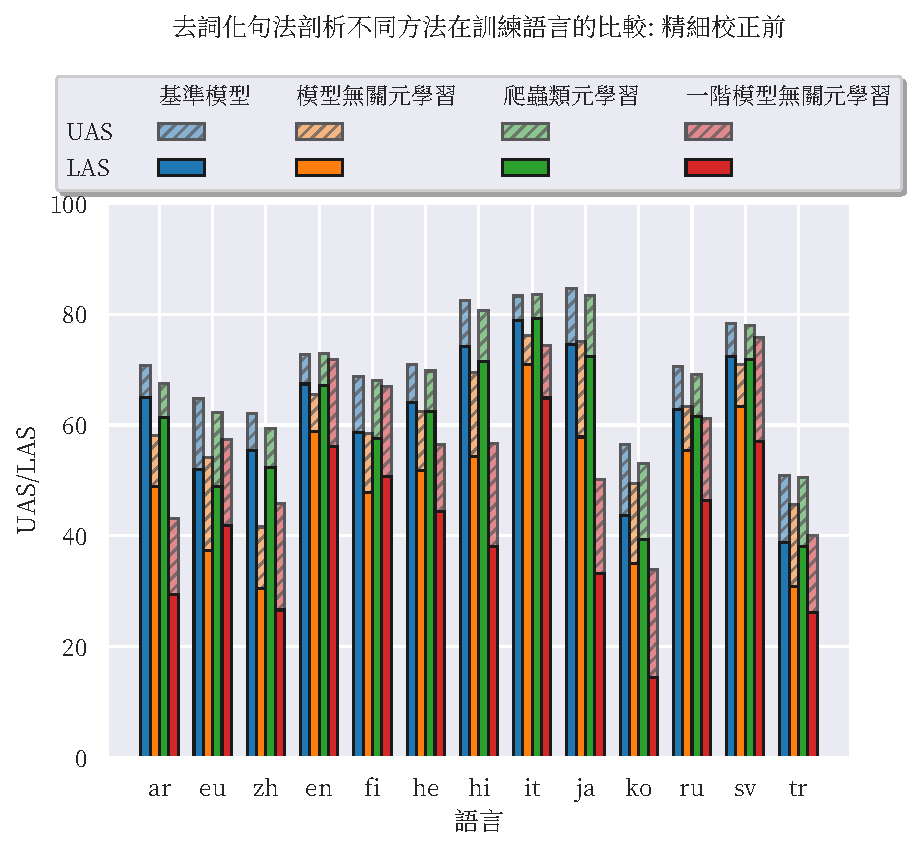
\includegraphics[width=\textwidth]{figs/chapter3/delex/bar_zs_train_langs.pdf}
    \end{subfigure}
    \vspace{-12pt}
    \begin{subfigure}[t]{0.8\textwidth}
        \centering
        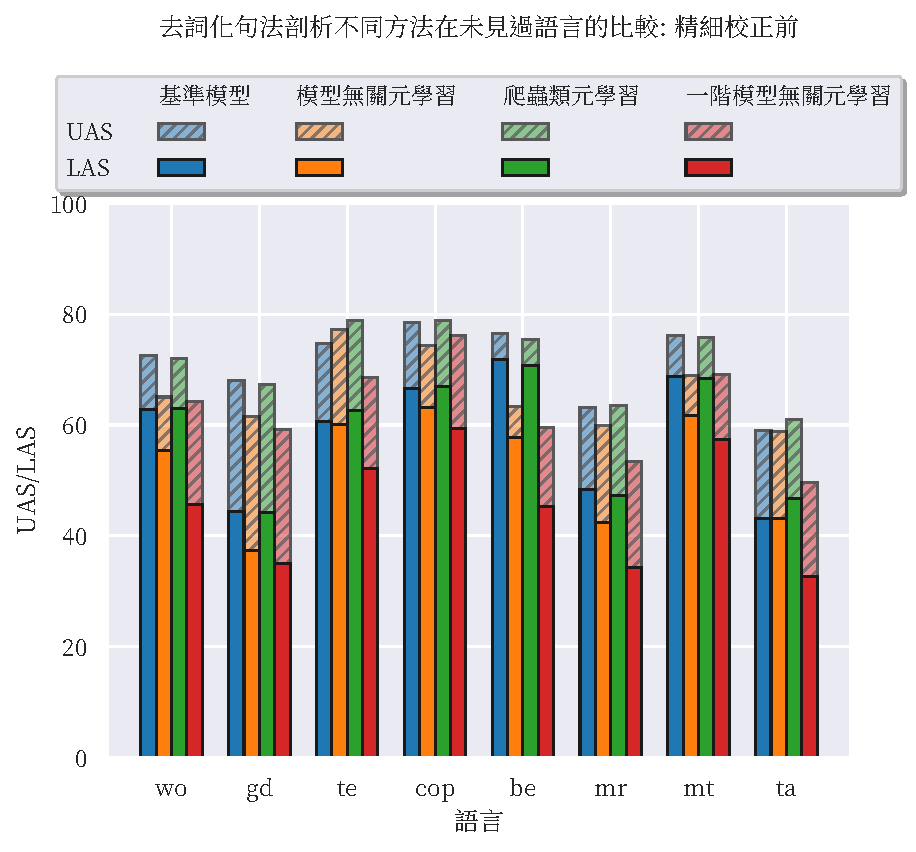
\includegraphics[width=\textwidth]{figs/chapter3/delex/bar_zs_test_langs.pdf}
    \end{subfigure}
    \caption{去詞化分析不同方法在各語言精細校正前的表現。}
    \label{fig:bar_zs}
\end{figure}
\begin{figure}[!htbp]
    \centering
    \begin{subfigure}[t]{0.75\textwidth}
        \centering
        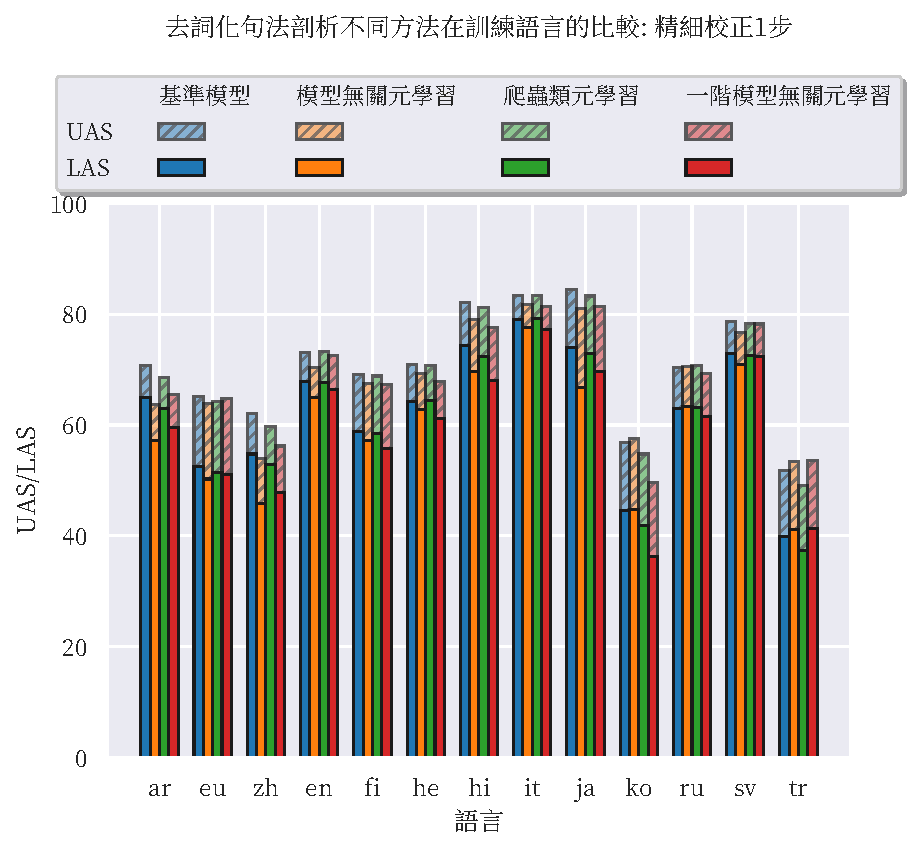
\includegraphics[width=\textwidth]{figs/chapter3/delex/bar_one_step_train_langs.pdf}
    \end{subfigure}
    \vspace{-12pt}
    \begin{subfigure}[t]{0.75\textwidth}
        \centering
        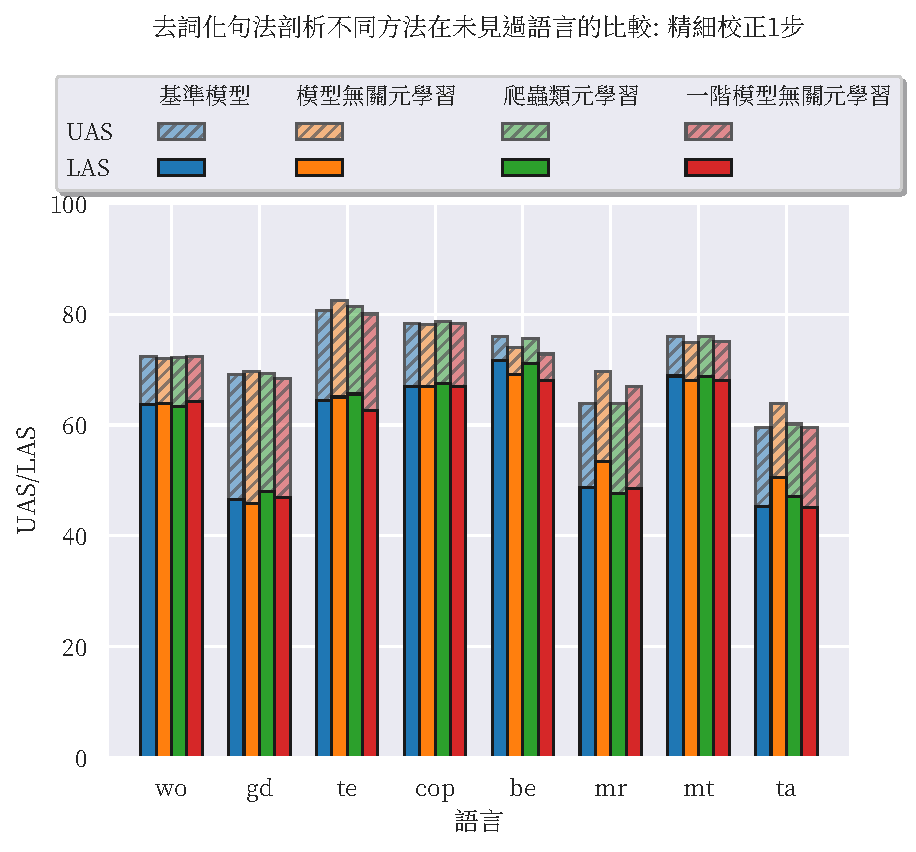
\includegraphics[width=\textwidth]{figs/chapter3/delex/bar_one_step_test_langs.pdf}
    \end{subfigure}
    \caption{去詞化分析不同方法在各語言精細校正一步($\frac{1}{6}$回合)後的表現。}
    \label{fig:bar_one_step}
\end{figure}
\begin{figure}[!htbp]
    \centering
    \begin{subfigure}[t]{0.75\textwidth}
        \centering
        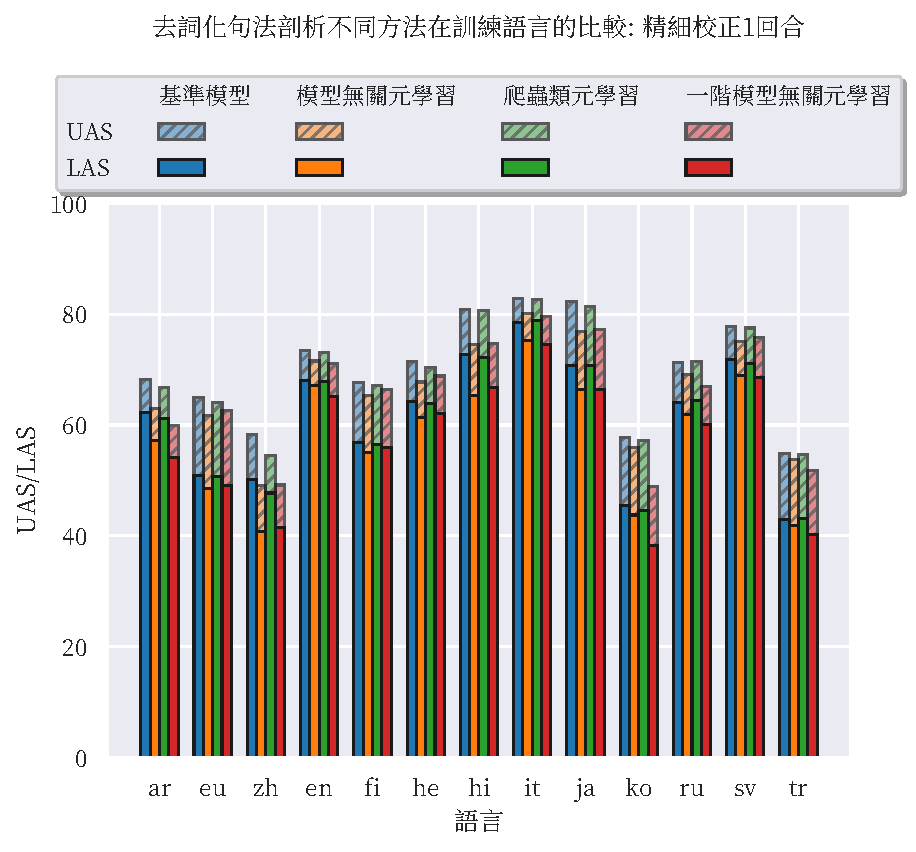
\includegraphics[width=\textwidth]{figs/chapter3/delex/bar_full_epoch_1_train_langs.pdf}
    \end{subfigure}
    \vspace{-12pt}
    \begin{subfigure}[t]{0.75\textwidth}
        \centering
        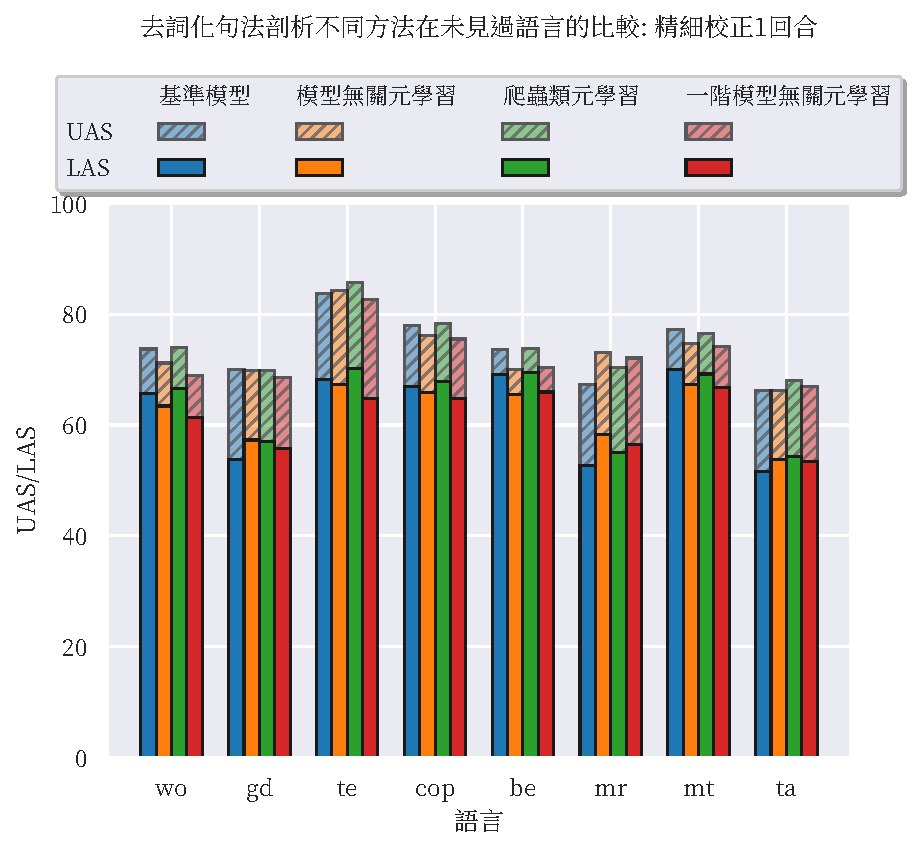
\includegraphics[width=\textwidth]{figs/chapter3/delex/bar_full_epoch_1_test_langs.pdf}
    \end{subfigure}
    \caption{去詞化分析不同方法在各語言精細校正一回合後的表現。}
    \label{fig:bar_full_epoch_1}
\end{figure}
\begin{figure}[htbp]
    \centering
    \begin{subfigure}[t]{0.8\textwidth}
        \centering
        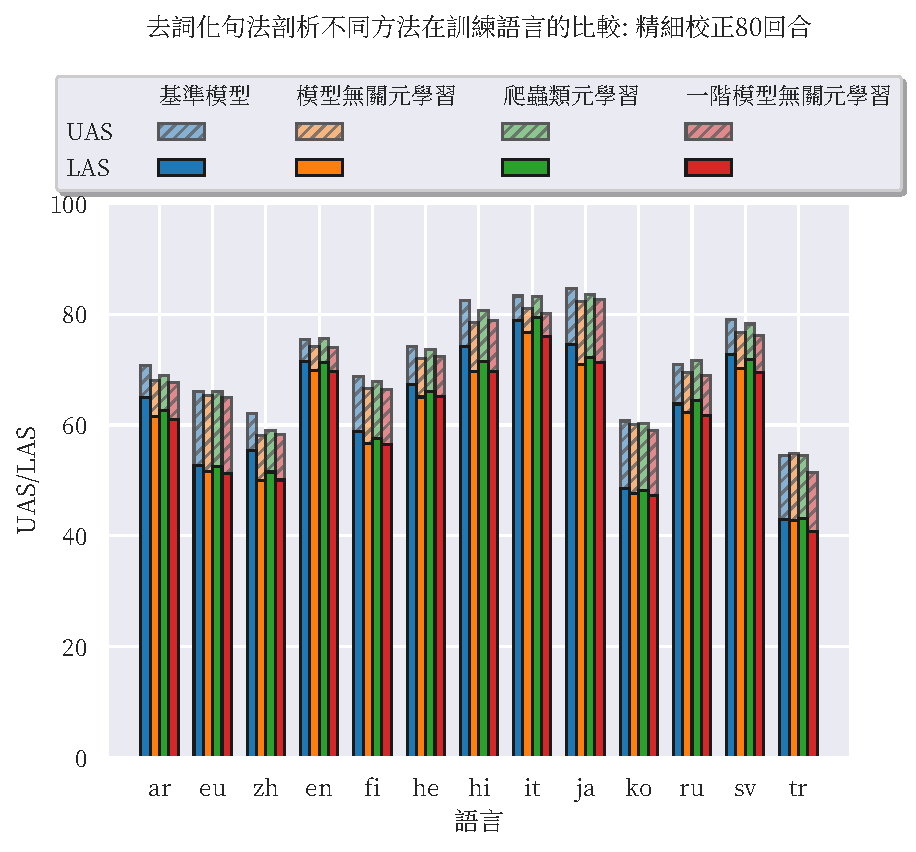
\includegraphics[width=\textwidth]{figs/chapter3/delex/bar_full_epoch_80_train_langs.pdf}
    \end{subfigure}
    \vspace{-12pt}
    \begin{subfigure}[t]{0.8\textwidth}
        \centering
        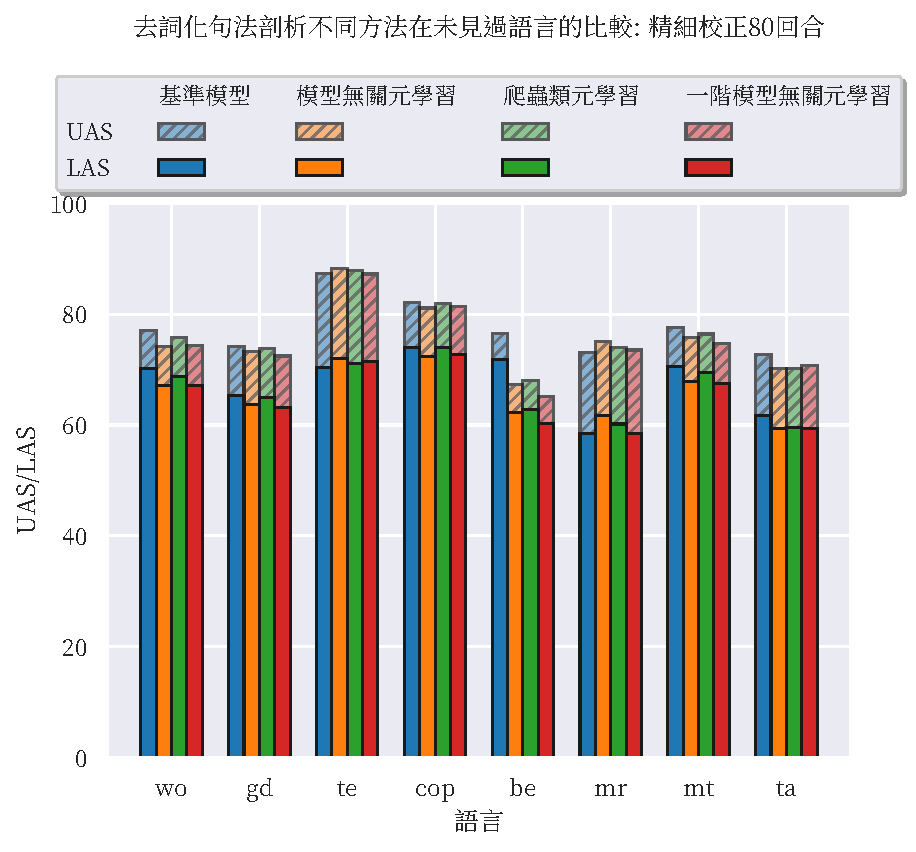
\includegraphics[width=\textwidth]{figs/chapter3/delex/bar_full_epoch_80_test_langs.pdf}
    \end{subfigure}
    \caption{去詞化分析不同方法在各語言精細校正八十回合後的表現。}
    \label{fig:bar_full_epoch_80}
\end{figure}
\pagebreak
\subsubsection{各預訓練方法不同內循環步數的比較}
\begin{figure}[!htbp]
    \centering
    \vspace{30pt}
    \begin{subfigure}[b]{0.8\textwidth}
        \centering
        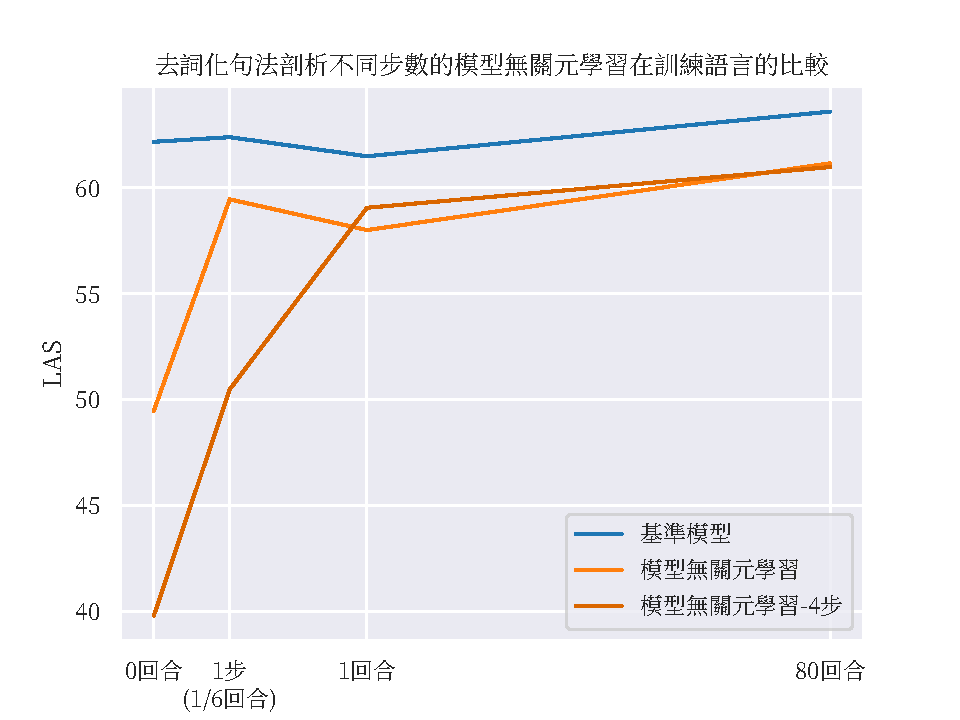
\includegraphics[width=\textwidth]{figs/chapter3/delex/delex_maml_train_langs.pdf}
    \end{subfigure}
    %\vspace{-12pt}
    \begin{subfigure}[b]{0.8\textwidth}
        \centering
        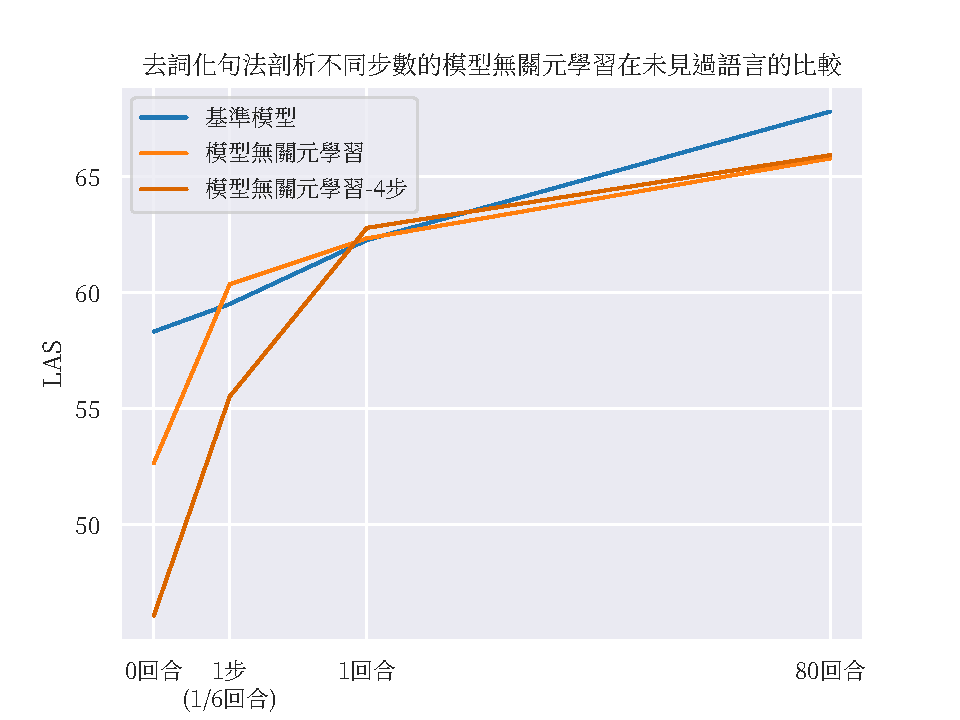
\includegraphics[width=\textwidth]{figs/chapter3/delex/delex_maml_test_langs.pdf}
    \end{subfigure}
    \caption{去詞化分析不同步數的模型無關元學習精細校正後在測試集上的平均表現。}
    \label{fig:delex_avg}
\end{figure}
\begin{figure}[htbp]
    \centering
    \begin{subfigure}[t]{\textwidth}
        \centering
        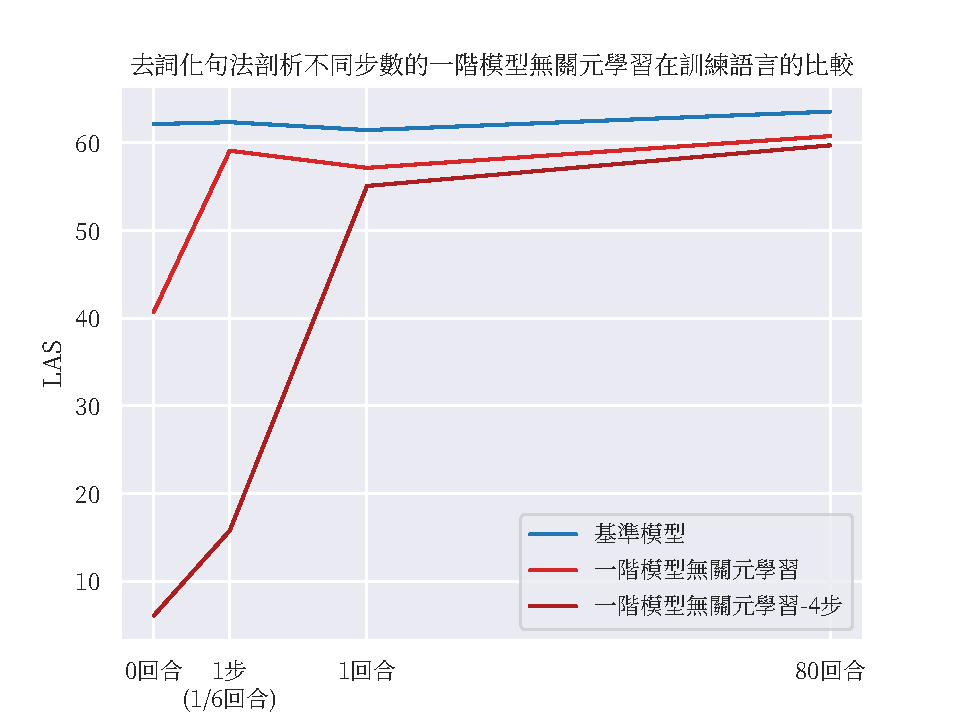
\includegraphics[width=\textwidth]{figs/chapter3/delex/delex_fomaml_train_langs.pdf}
    \end{subfigure}
    \vspace{-12pt}
    \begin{subfigure}[t]{\textwidth}
        \centering
        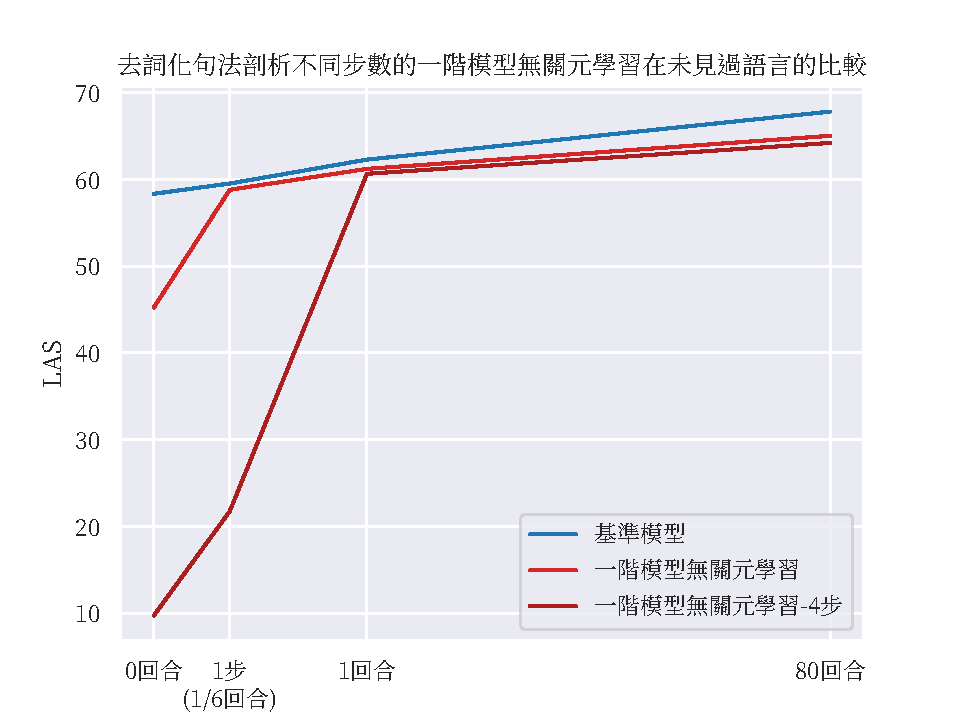
\includegraphics[width=\textwidth]{figs/chapter3/delex/delex_fomaml_test_langs.pdf}
    \end{subfigure}
    \caption{去詞化分析不同步數的一階模型無關元學習精細校正後在測試集上的平均表現。}
    \label{fig:delex_avg}
\end{figure}
\begin{figure}[htbp]
    \centering
    \begin{subfigure}[t]{\textwidth}
        \centering
        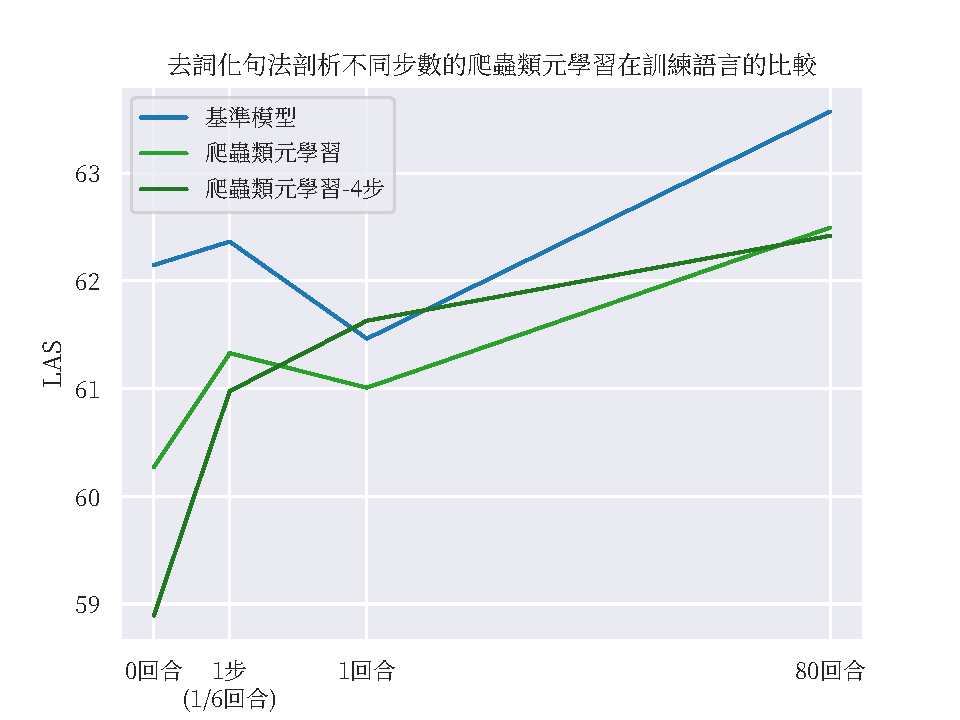
\includegraphics[width=390pt]{figs/chapter3/delex/delex_reptile_train_langs.pdf}
    \end{subfigure}
    \vspace{-12pt}
    \begin{subfigure}[t]{\textwidth}
        \centering
        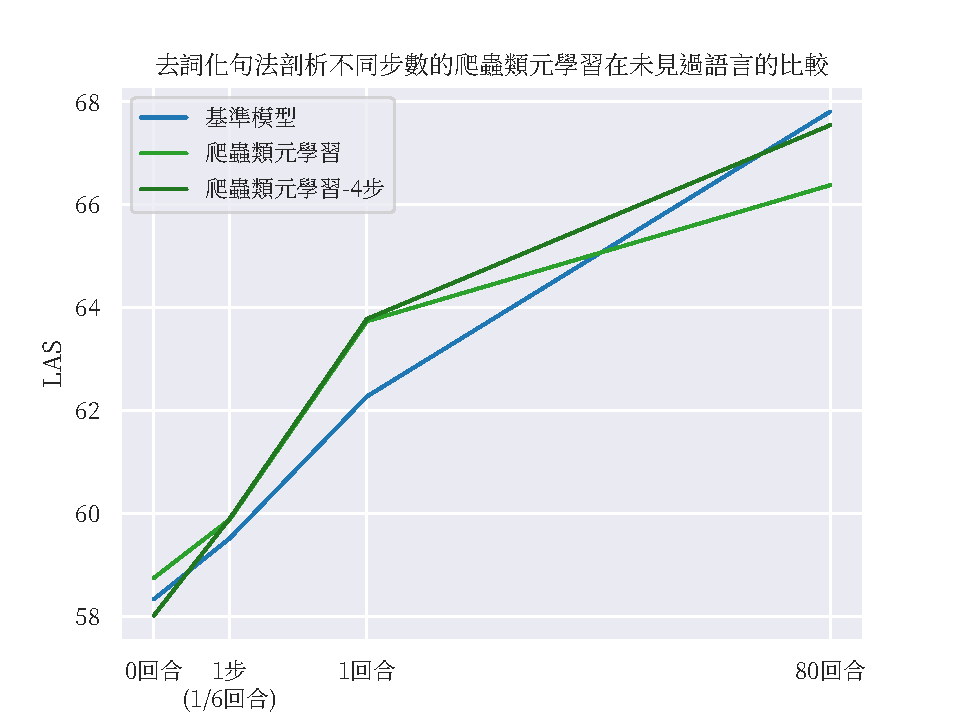
\includegraphics[width=390pt]{figs/chapter3/delex/delex_reptile_test_langs.pdf}
    \end{subfigure}
    \caption{去詞化分析不同步數的爬蟲類元學習精細校正後在測試集上的平均表現。}
    \label{fig:delex_avg}
\end{figure}
\pagebreak
\subsubsection{小模型下各預訓練方法的比較}
\begin{figure}[!htbp]
    \centering
    \begin{subfigure}[t]{0.75\textwidth}
        \centering
        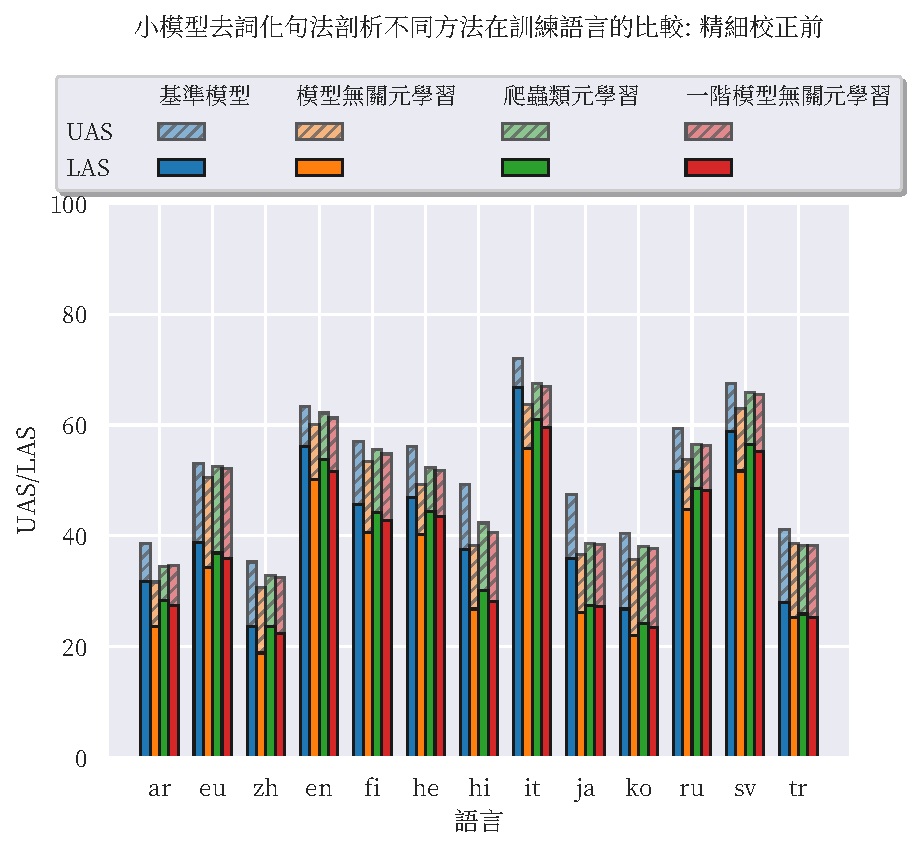
\includegraphics[width=\textwidth]{figs/chapter3/delex/bar_small_zs_train_langs.pdf}
    \end{subfigure}
    \vspace{-12pt}
    \begin{subfigure}[t]{0.75\textwidth}
        \centering
        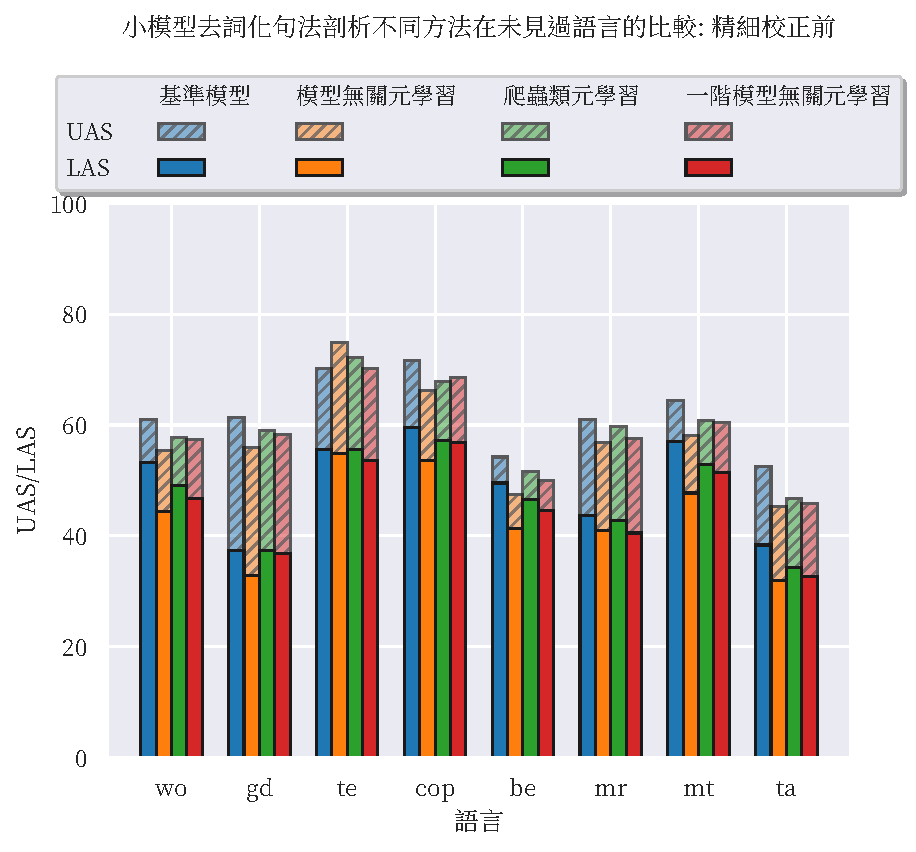
\includegraphics[width=\textwidth]{figs/chapter3/delex/bar_small_zs_test_langs.pdf}
    \end{subfigure}
    \caption{小模型去詞化分析不同方法在各語言精細校正前的表現。}
    \label{fig:bar_small_zs}
\end{figure}
\begin{figure}[!htbp]
    \centering
    \begin{subfigure}[t]{0.75\textwidth}
        \centering
        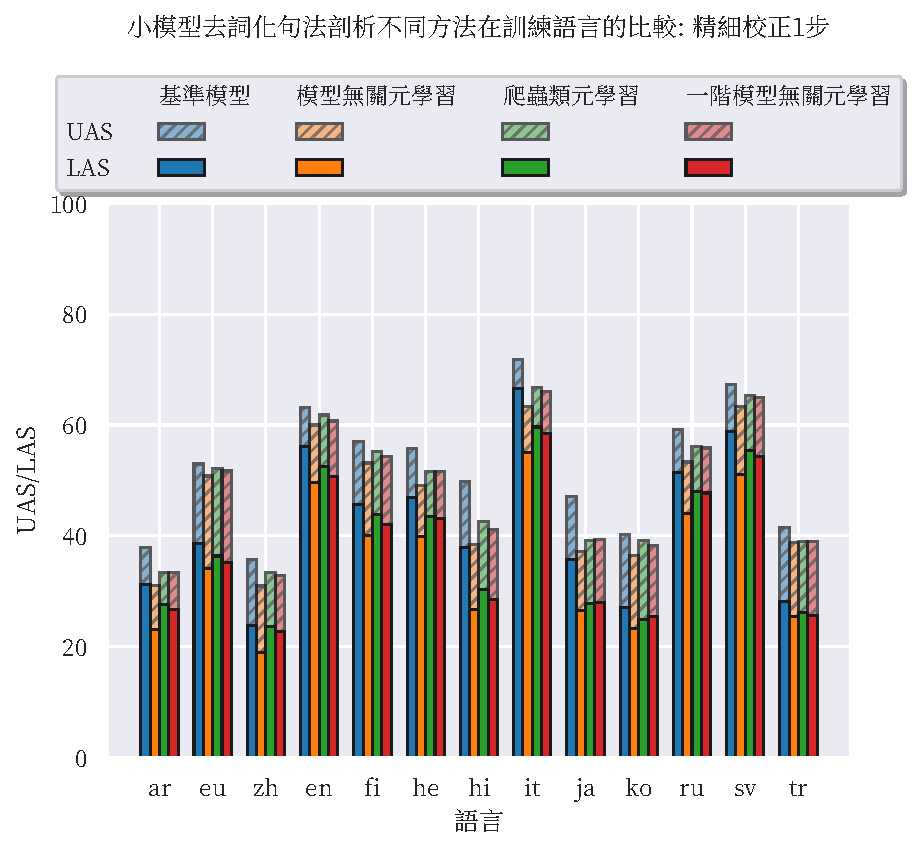
\includegraphics[width=\textwidth]{figs/chapter3/delex/bar_small_one_step_train_langs.pdf}
    \end{subfigure}
    \vspace{-12pt}
    \begin{subfigure}[t]{0.75\textwidth}
        \centering
        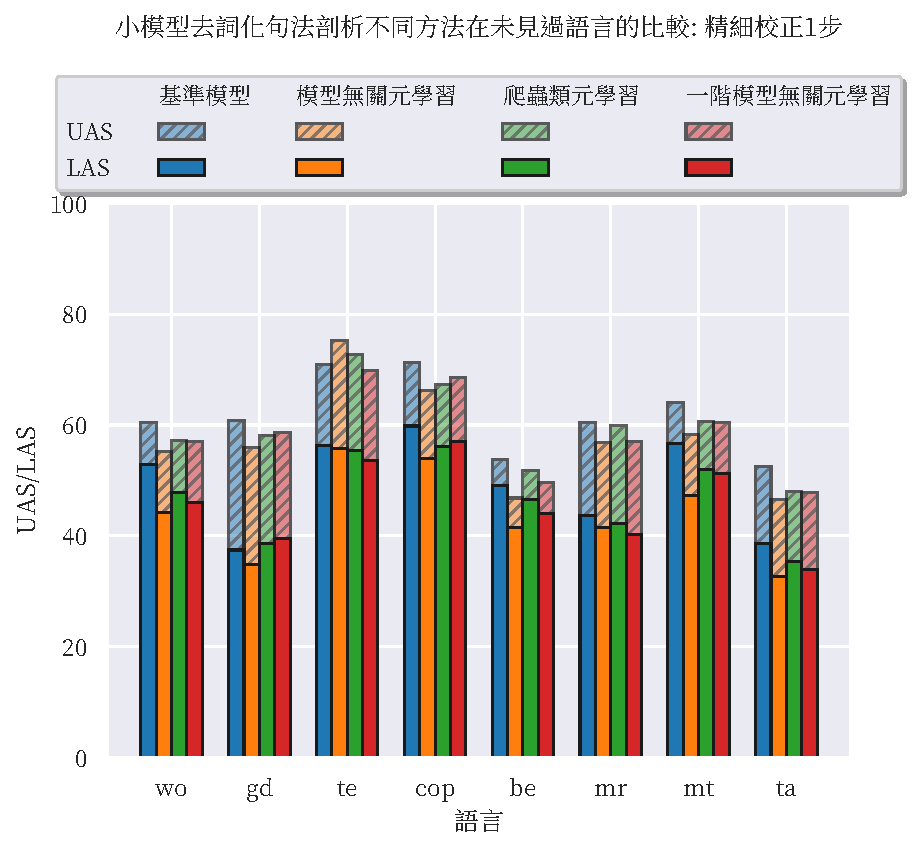
\includegraphics[width=\textwidth]{figs/chapter3/delex/bar_small_one_step_test_langs.pdf}
    \end{subfigure}
    \caption{小模型去詞化分析不同方法在各語言精細校正一步($\frac{1}{6}$回合)後的表現。}
    \label{fig:bar_small_one_step}
\end{figure}
\begin{figure}[htbp]
    \centering
    \begin{subfigure}[t]{0.8\textwidth}
        \centering
        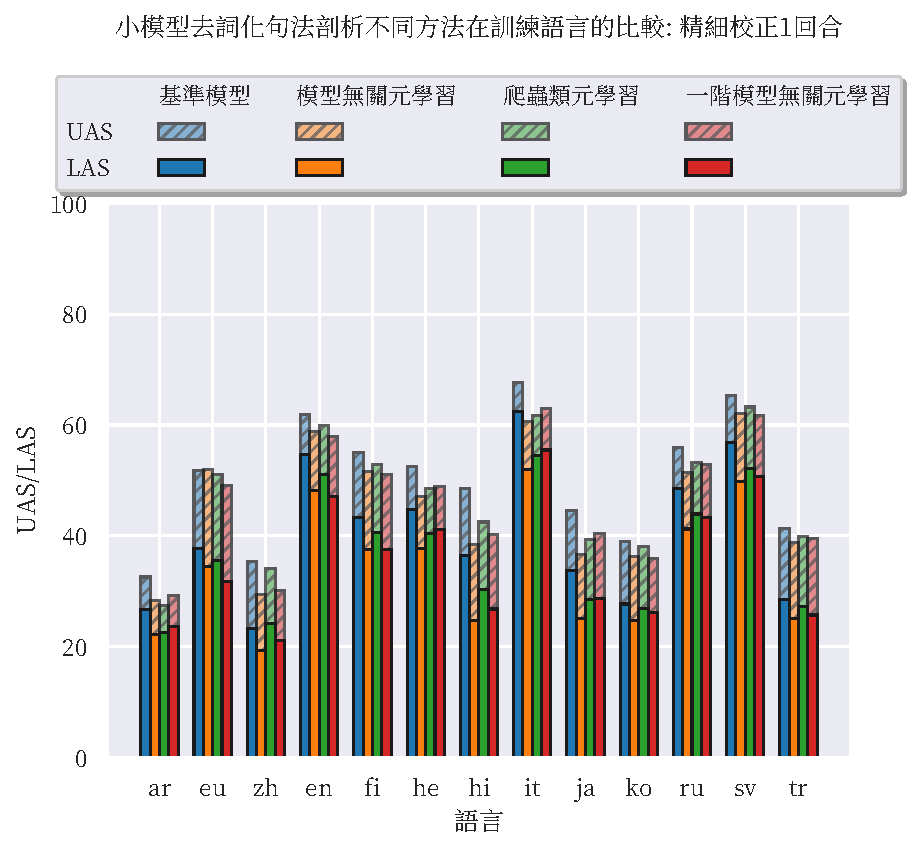
\includegraphics[width=\textwidth]{figs/chapter3/delex/bar_small_full_epoch_1_train_langs.pdf}
    \end{subfigure}
    \vspace{-12pt}
    \begin{subfigure}[t]{0.8\textwidth}
        \centering
        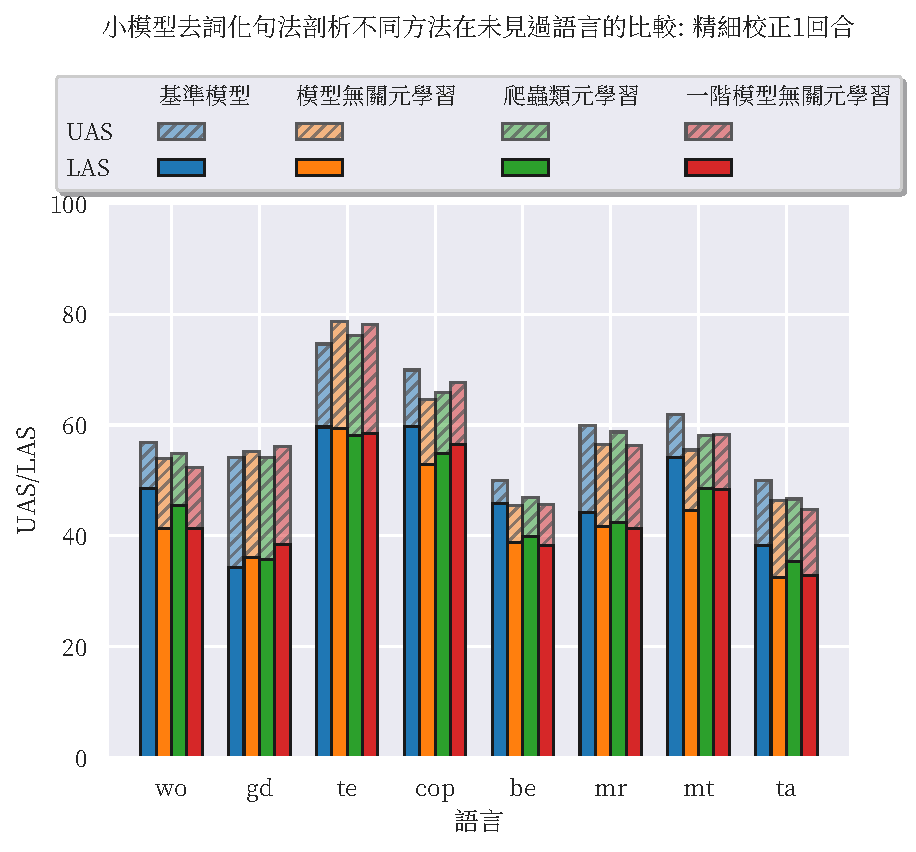
\includegraphics[width=\textwidth]{figs/chapter3/delex/bar_small_full_epoch_1_test_langs.pdf}
    \end{subfigure}
    \caption{小模型去詞化分析不同方法在各語言精細校正一回合後的表現。}
    \label{fig:bar_small_full_epoch_1}
\end{figure}
\begin{figure}[!htbp]
    \centering
    \begin{subfigure}[t]{0.75\textwidth}
        \centering
        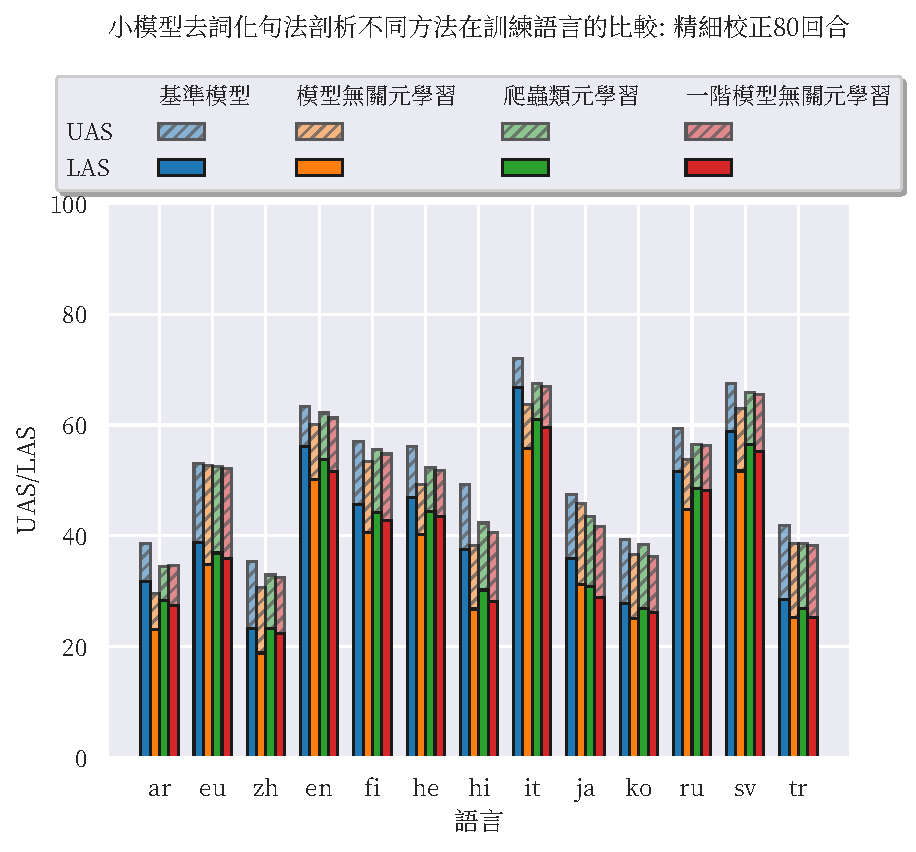
\includegraphics[width=\textwidth]{figs/chapter3/delex/bar_small_full_epoch_80_train_langs.pdf}
    \end{subfigure}
    \vspace{-12pt}
    \begin{subfigure}[t]{0.75\textwidth}
        \centering
        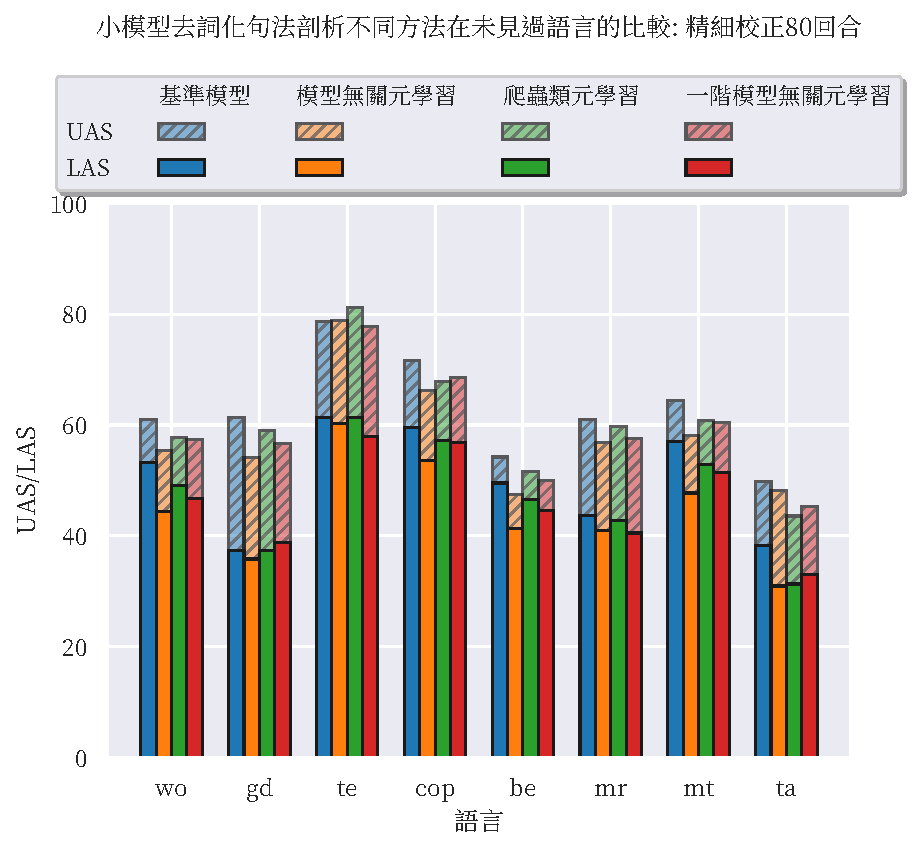
\includegraphics[width=\textwidth]{figs/chapter3/delex/bar_small_full_epoch_80_test_langs.pdf}
    \end{subfigure}
    \caption{小模型去詞化分析不同方法在各語言精細校正八十回合後的表現。}
    \label{fig:bar_small_full_epoch_80}
\end{figure}

%\subsection{限制}
%去詞化分析使用普適詞性標注在多語言句法剖析中,雖然排除了各個語言句法以外性質對句法剖析的影響
\section{多語言依存句法分析(multilingual dependency parsing)}

\subsection{模型架構}

\subsubsection{圖類剖析器 -- 深層雙仿射層注意力網路(Graph-based Parser -- Deep Biaffine Attention)}

2017年由多氏\cite{Dozat2017DeepBA}提出的深層雙仿射層注意力網路(下稱\textbf{雙仿射}),憑藉其簡單的模型架構及強大的實務表現,成爲近年來最常被採用的句法剖析模型。
與其他圖類剖析器一樣,\textbf{雙仿射}的目標為學習邊評分分數:$s(\MWord_{i}, \MWord_{j})$,使得正確句法樹出現的可能性提高。

給定編碼器函數$\MRep\left(\MWord\right) \in \mathbb{R}^{n}$、雙線性矩陣$\mathbf{U}^{(1)} \in \mathbb{R}^{n \times n}$、
線性矩陣$U^{(2)},\ U^{(3)} \in \mathbb{R}^{n} $與偏差$\mathbf{b}$,\textbf{雙仿射}的邊評分函數為:
\begin{equation}
    s(\MWord_{i}, \MWord_{j}) = \MRep(\MWord_{i})^{\top} \mathbf{U}^{(1)} \MRep(\MWord_{j}) + \MRep(\MWord_{i})^{\top} U^{(2)} + \MRep(\MWord_{j})^{\top} U^{(3)} + \mathbf{b}\ .
\end{equation}
上式可分為三部分解釋:$\MRep(\MWord_{i})^{\top} U^{(2)}$代表$w_{i}$接受任何子節點的可能性;$\MRep(\MWord_{j})^{\top} U^{(3)}$代表$w_{j}$接受任何父節點的可能性;
$\MRep(\MWord_{i})^{\top} \mathbf{U}^{(1)} \MRep(\MWord_{j})$則代表$\MWord_{i}$與$\MWord_{j}$之間存在連結(邊)的可能性。

\subsubsection{多語言基於轉換器模型的雙向編碼器表示(multilingual BERT)}

句法剖析的架構中,在大型預訓練語言模型出現以前,編碼器函數$\MRep\left(\MWord\right)$常見的選擇為數層隨機初始化的LSTM或轉換器;
大型預訓練語言模型出現後,以其為編碼器函數的初始訓練參數進行精細校正(fine-tuning)所訓練出的剖析器紛紛取得更好的成績。
多語言的句法剖析在大型預訓練語言模型出現之前較少文獻直接讓各語言共同分享編碼器函數,
真正共享參數的也多為接受詞性標記而非文字的去詞化依存句法剖析(delexicalized dependency parsing),
其原因主要可歸結為多語言模型需要設計統一的記符集(token set)來表示每個語言各異的書寫系統(writing system)產生的文字。
在單語言時可直接用該語言經斷詞後所統計出的常見詞作為記符(token);
單語言的常見詞數目通常設定在10000-40000詞即非常堪用,剩下的低頻詞並不影響模型表現太多;
但多語言模型若不減少任一語言之記符數而直接結合各語言的詞彙做為記符集,此記符集將變得太大,且相近語言無法透過相似的構詞共享參數,
如西班牙文的「學生」一詞``estudiante''與其英文的對應``student''有共同的詞子字串``stud'',上述直接結合的方法便無法讓模型學習到這些共通性。
文獻上已經提出許多解決辦法,以下列舉三項:
\begin{itemize}
    \item 使用語素分割器(morpheme segmenter):利用專家知識構造出基於規則或統計的語素分割器分割語素,並以語素為記符,分割結果符合人類知識,
使相似詞可以正確的共用語素記符向量的參數爲其優點,
惟某些語言可能不存在準確率高的語素分割器,通用性不足。
    \item 使用字符(character)做為記符:優點為不需要某些語言可能沒有的語素分割器,但字符顆粒度過小,單句話的記符數變多,會增加模型處理時間。
    \item 使用次級詞分割(subword tokenization)演算法:次級詞是比詞小但比字符大的記符,
由演算法統計出語言中的詞彙較常獨立出現的子字串(substring)做為新的記符,將詞取代為多個子字串的結合,也可看做是非監督式演算法計算出的語素。
常見的演算法包括字節對編碼(Byte-pair encoding)~\cite{sennrich-etal-2016-neural}、WordPiece \cite{schuster2012japanese}等。
\end{itemize}
其中次級詞雖然分割品質受演算法及訓練語料大小影響良窳不一,但其兼備語素分割器共用子字串與字符不需要人類知識的優點,
因此現行單語言與多語言的大型預訓練語言模型均採用次級詞做為記符來取代原本以詞或字符為單位的表示法。

本研究與目前孔氏提出的多語言句法剖析的最佳單一模型Udify\cite{kondratyuk-straka-2019-75}
一樣採用\textbf{多語言基於轉換器模型的雙向編碼器表示}(下稱$\mathrm{mBERT}$)作為編碼器函數來編碼語料中的衆多語言。

令 $\MRep\left(\MWord\right)$ 為編碼器函數,
$\mathrm{mBERT}\left(\MWord\right)_{i}$為記符$\MWord$通過$\mathrm{mBERT}$第$i$層的輸出,
由於許多文獻\cite{peters-etal-2018-deep,devlin-etal-2019-bert}均指出與其讓下游任務只接受最後一層的輸出,
讓模型在精細校正(fine-tuning)時自由混合幫助較大的輸出層更有助於模型表現,
而特氏也發現\cite{tenney-etal-2019-bert}若交由每個任務自由混合預訓練模型不同層數的輸出,
不同任務所給予的層權重分佈大不相同,其中與句法相關的任務(如詞性標註、句法標註)傾向給予接近輸入的層較大的權重,
而與語意相關的任務則給予接近輸出的層較大的權重,顯示原本只取最後一層的方法恐非最佳策略;
因此這裏採用彼氏(Matthew Peters)提出的層專注機制(layer attention),
給予每一層輸出專注權重,
讓模型決定哪一層的輸出對句法剖析較有幫助:

\begin{equation}
    \MRep\left(\MWord\right) = \alpha \sum_{i=1}^{L} \mathrm{mBERT}\left(\MWord\right)_{i} \cdot \mathrm{softmax} {\left(\mathbf{c}\right)}_{i}
\end{equation}
其中$L$為$\mathrm{mBERT}$的層數(本研究使用\texttt{bert-base-multilingual-cased}版本\footnote{見\url{https://github.com/google-research/bert}},$L=12$),
$\alpha$為可調整的純量,$\mathbf{c} \in \mathbb{R}^{L}$為層專注權重。

為了防止模型過於仰賴特定層的資訊而造成過擬合,這裏採用孔氏提出的\cite{kondratyuk-straka-2019-75}的層丟棄(layer dropout),
在訓練時每個層專注權重$c_{i}$有$p=0.1$的機率被設為$-\infty$,使權重重新分配到其他的層上,
迫使模型整合$\mathrm{mBERT}$全部層輸出的資訊,而非偏重特定某幾層。

\subsubsection{適應器(adapter)}

適應器為雷氏(Sylvestre-Alvise Rebuffi)\cite{rebuffi2018efficient}所提出在影像領域的轉移學習方法,
後由何氏(Neil Houlsby)引進自然語言處理常用的轉換器模型\cite{houlsby2019parameter},
其指出當時自然語言處理的轉移學習方法多半使用大型預訓練轉換器模型進行全模型精細校正在目標任務上,
但何氏認為全模型精細校正需要調整模型中所有的參數,每種任務都會產生一個全新的模型,
太耗費儲存空間與計算資源,且大型預訓練轉換器模型已經含有大量句法語意等任務所需資訊,應不需要變動參數過多;
因此他提出固定原本的大型預訓練轉換器模型參數,但在被固定的模型層中加入具殘差網路性質的適應器,
模型只需為每個任務調整適應器少量的參數,任務間還是共享原本的大型預訓練轉換器模型參數,
而實驗數據也顯示,加入適應器的轉換器模型可以在所需調整的參數量遠低於全模型精細校正下,在目標任務中達成與其相似的表現。
其架構為一前饋層組成的兩層瓶頸網路(一層投射到較小維度,一層投射回原本維度),
再加上殘差連結(residual),置於轉換器中前饋層後、層\XNorm之前的位置,細節可見圖\ref{fig:adapter}。
%其指出學習一通用特徵抽取器(universal feature extractor),
%然後在其後為每個任務接上一個任務專屬模組(task-specific module)做精細校正,
%這樣的方法雖然可以充分利用通用特徵抽取器的精緻特徵一次解決多個任務,但其各自任務的表現通常沒有專精單一任務來得好;
%因此他提出在通用特徵抽取器
\begin{figure}[htbp]
    \centering
    \begin{subfigure}[t]{0.5\textwidth}
        \centering
        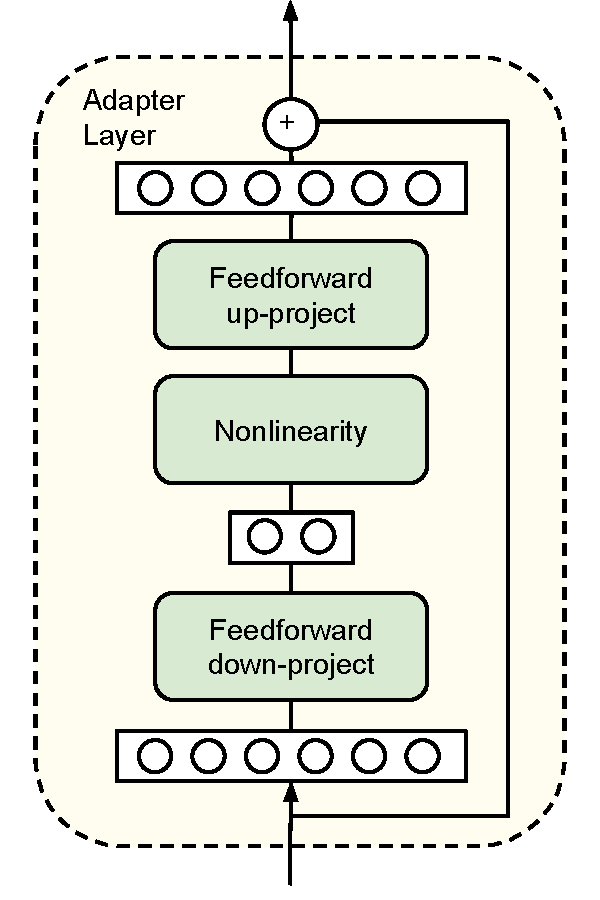
\includegraphics[width=\textwidth]{figs/chapter3/adapters/adapter_arch.pdf}
    \end{subfigure}%
    \begin{subfigure}[t]{0.5\textwidth}
        \centering
        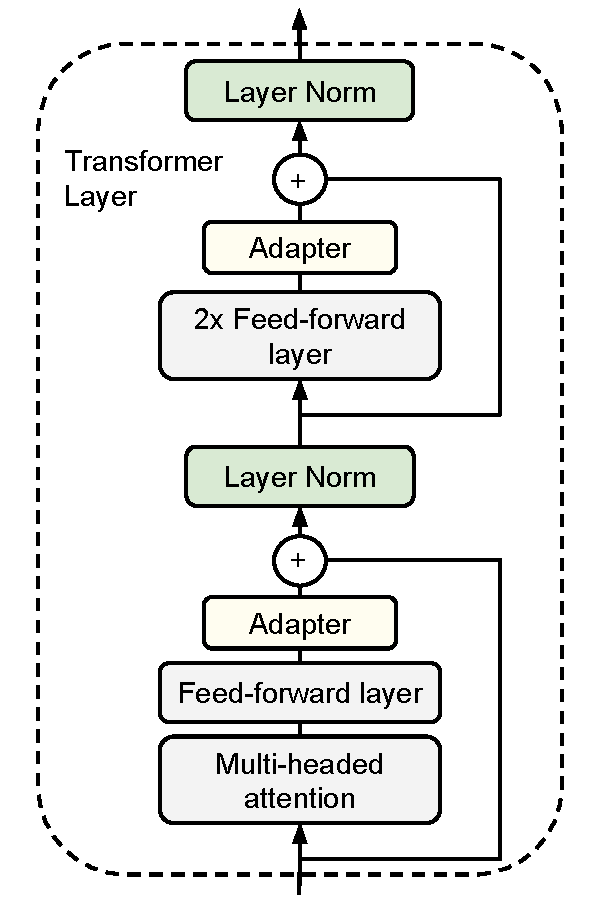
\includegraphics[width=\textwidth]{figs/chapter3/adapters/adapter_insertion.pdf}
        %\caption{加入適應器後的轉換器架構(圖取自\cite{rebuffi2018efficient})。}
    \end{subfigure}
    \caption{\textbf{左側}:適應器架構;\textbf{右側}:加入適應器後的轉換器架構(圖取自\cite{rebuffi2018efficient})。}
    \label{fig:adapter}
\end{figure}
%\input{figs/chapter3/adapters/adapter_ins.tex}

\subsection{實驗設置}

\subsubsection{基準模型與元學習模型共同實驗設置}

本節的實驗設置基於\conll 的實驗設置,但做了些微改變:
我們從\conll 的53種訓練語言(73個訓練句法樹庫)中選取有官方驗證集(development set)的46種訓練語言(66個訓練句法樹庫)作爲訓練語言;見表\ref{tab:training_languages}。
預訓練完成後,我們分別對該模型進行\zeroshot 及\finetune 在預訓練中未見過的語言上。
本節實驗在訓練語言與測試語言的切分與章節\ref{subsec:delex_depparse_setting}去詞化的依存句法剖析設置大致相同,不再贅述,
而訓練方法部分,
在訓練時也均使用正確的斷句、斷詞,
惟測試時爲了與\conll 相比,由於\conll 連句法剖析之前的預處理(斷句、斷詞)也納入整體評分,
但研究重點在句法剖析而非預處理,
因此直接採用StanfordNLP的預處理系統\cite{qi-etal-2018-universal}\footnote{https://github.com/stanfordnlp/stanfordnlp}。

%孔氏\cite{kondratyuk-straka-2019-75}與烏氏\cite{ustun2020udapter}進行多語言訓練的方法,是將全部語言的句法樹庫接在一起、在一個小批次(batch)中混合多個句法樹庫訓練。
%這樣的做法可能會導致資料量大的語言取樣頻率過高;我們的方法則是每次更新從全部語言裡取樣$l$種語言,每種語言取樣$b$個句子,一個批次總共有$b \times l$個句子。
%不同於孔氏與烏氏,這樣的方法防止模型過度對資料充足語言的特性建模,但也可能使得資料不足語言的句子被過度取樣而產生過擬合的現象。

本研究跟隨烏氏的做法,採用適應器模型\finetune $\mathrm{mBERT}$在依存句法剖析任務上。
除了優化器的暖身步數因更改批次大小而跟着更改以外,大部分的超參數都與烏氏的設置一樣;見表\ref{tab:pretrain_hparams}。

其他設置均與章節\ref{subsec:delex_depparse_setting}所述相同。

\subsubsection{元學習實驗設置}

對於\reptile 與\fomaml ,如無特別註明,外迴圈學習率(outer-loop learning rate)與內迴圈學習率(inner loop-learning rate)相同。
\subsubsection{\zeroshot (Zero-shot Transfer)實驗設置}
我們選取CoNLL 2018 Shared Task中只有訓練集而沒有發展集的語言作爲測試語言。

\begin{table}[h!]
\centering
\begin{subtable}[t]{.5\textwidth}
    \begin{tabular}[t]{|l l|}
        \hline
        \textbf{語言} & \textbf{句法樹庫編碼} \\
        \hline
        Afrikaans & af\_afribooms \\
        Ancient Greek & grc\_proiel \\
        Ancient Greek & grc\_perseus \\
        Arabic & ar\_padt \\
        %Armenian & hy\_armtdp \\
        Basque & eu\_bdt \\
        Bulgarian & bg\_btb \\
        %Buryat & bxr\_bdt \\
        Catalan & ca\_ancora \\
        Chinese & zh\_gsd \\
        Croatian & hr\_set \\
        Czech & cs\_cac \\
        Czech & cs\_fictree \\
        Czech & cs\_pdt \\
        Danish & da\_ddt \\
        Dutch & nl\_alpino \\
        Dutch & nl\_lassysmall \\
        English & en\_ewt \\
        English & en\_gum \\
        English & en\_lines \\
        Estonian & et\_edt \\
        Finnish & fi\_ftb \\
        Finnish & fi\_tdt \\
        French & fr\_gsd \\
        French & fr\_sequoia \\
        French & fr\_spoken \\
        Galician & gl\_ctg \\
        Galician & gl\_treegal \\
        German & de\_gsd \\
        Gothic & got\_proiel \\
        Greek & el\_gdt \\
        Hebrew & he\_htb \\
        Hindi & hi\_hdtb \\
        Hungarian & hu\_szeged \\
        Indonesian & id\_gsd \\
        %Irish & ga\_idt \\
        \hline
    \end{tabular}
\end{subtable}%
\begin{subtable}[t]{.5\textwidth}
    \begin{tabular}[t]{|l l|}
        \hline
        \textbf{語言} & \textbf{句法樹庫編碼} \\
        \hline
        Italian & it\_isdt \\
        Italian & it\_postwita \\
        Japanese & ja\_gsd \\
        %Kazakh & kk\_ktb \\
        Korean & ko\_gsd \\
        Korean & ko\_kaist \\
        %Kurmanji & kmr\_mg \\
        Latin & la\_ittb \\
        Latin & la\_proiel \\
        Latin & la\_perseus \\
        Latvian & lv\_lvtb \\
        %North Sami & sme\_giella \\
        Norwegian & no\_bokmaal \\
        Norwegian & no\_nynorsk \\
        Norwegian & no\_nynorsklia \\
        Old Church Slavonic & cu\_proiel \\
        Old French & fro\_srcmf \\
        Persian & fa\_seraji \\
        Polish & pl\_lfg \\
        Polish & pl\_sz \\
        Portuguese & pt\_bosque \\
        Romanian & ro\_rrt \\
        Russian & ru\_syntagrus \\
        Russian & ru\_taiga \\
        Serbian & sr\_set \\
        Slovak & sk\_snk \\
        Slovenian & sl\_ssj \\
        Slovenian & sl\_sst \\
        Spanish & es\_ancora \\
        Swedish & sv\_lines \\
        Swedish & sv\_talbanken \\
        Turkish & tr\_imst \\
        Ukrainian & uk\_iu \\
        %Upper Sorbian & hsb\_ufal \\
        Urdu & ur\_udtb \\
        Uyghur & ug\_udt \\
        Vietnamese & vi\_vtb \\
        \hline
    \end{tabular}
\end{subtable}
\caption{預訓練所使用的訓練句法樹庫/語言。}
\label{tab:training_languages}
\end{table}
\begin{table}[h!]
\centering
\begin{subtable}[t]{.5\textwidth}
    \centering
    \begin{tabular}[t]{|l l|}
        \hline
        \textbf{語言} & \textbf{句法樹庫編碼} \\
        \hline
        Buryat & bxr\_bdt \\
        Kurmanji & kmr\_mg \\
        Upper Sorbian & hsb\_ufal \\
        Armenian & hy\_armtdp \\
        Kazakh & kk\_ktb \\
        Irish & ga\_idt \\
        North Sami & sme\_giella \\
        \hline
    \end{tabular}
    \caption{真實資料不足測試句法樹庫/語言。}
    \label{tab:true_lr_testing_languages}
\end{subtable}%
\begin{subtable}[t]{.5\textwidth}
    \centering
    \begin{tabular}[t]{|l l|}
        \hline
        \textbf{語言} & \textbf{句法樹庫編碼} \\
        \hline
        Wolof & wo\_wtb \\
        Scottish Gaelic & gd\_arcosg \\
        Coptic & cop\_scriptorium \\
        Telugu & te\_mtg \\
        Belarusian & be\_hse \\
        Marathi & mr\_ufal \\
        Maltese & mt\_mudt \\
        Tamil & ta\_ttb \\
        \hline
    \end{tabular}
    \caption{模擬資料不足測試句法樹庫/語言。}
    \label{tab:sim_lr_testing_languages}
\end{subtable}%
\caption{資料不足測試句法樹庫/語言。}
\end{table}
\begin{table}[htbp]
    % \fontsize{8}{10}\selectfont
    \centering
    \begin{subtable}[t]{.4\textwidth}
        \begin{tabular}[t]{@{}lr@{}}
        \toprule
        超參數 & 值 \\
        \midrule
            依存標籤維度         & 256 \\
            依存邊維度           & 768 \\
            丟棄機率            & 0.5 \\
            BERT丟棄機率        & 0.2 \\
            BERT遮蔽機率        & 0.2 \\
            層丟棄機率          & 0.1 \\
            批次大小$b$         & 16 \\
            語言數$l$           & 10 \\
            訓練樣本數/回合        & 64000 \\
            訓練回合數          & 10 \\
            優化器              & Adam \\
            $\beta_1,\beta_2$  & 0.9, 0.99 \\
            權重衰減參數         & 0.01 \\
            基礎學習率          & $1e^{-3}$ \\
            學習率調度器        & ulmfit\_sqrt \\
            學習率暖身步數       & 1231 \\
            最大梯度範數        & 5.0 \\
        \bottomrule
        \end{tabular}
        \caption{
            預訓練超參數。
        }
        \label{tab:pretrain_hparams}
    \end{subtable}
    \begin{subtable}[t]{.4\textwidth}
        \begin{tabular}[t]{@{}lr@{}}
        \toprule
        超參數 & 值 \\
        \midrule
            丟棄機率            & 0.5 \\
            BERT丟棄機率        & 0.2 \\
            BERT遮蔽機率        & 0.2 \\
            層丟棄機率          & 0.1 \\
            批次大小            & 8 \\
            訓練回合數          & 80 \\
            優化器              & Adam \\
            $\beta_1,\beta_2$  & 0.9, 0.99 \\
            權重衰減參數         & 0.01 \\
            基礎學習率          & $5e^{-5}$ \\
            學習率調度器        & slanted\_triangular \\
            學習率暖身步數       & 1(回合)\\
            最大梯度範數        & 5.0 \\
            交叉驗證摺數$k$     & 3   \\
        \bottomrule
        \end{tabular}
        \caption{
            精細校正超參數。
        }
        \label{tab:finetune_hparams}
    \end{subtable}
    \caption{
        模型超參數一覽。
    }
    \label{tab:hparams}
\end{table}

\subsubsection{\finetune (Fine-tuning)實驗設置}
本論文從預訓練完的模型開始對目標語言\finetune 40個回合。其他\finetune 的超參數請見表\ref{tab:finetune_hparams}。

由於選取的測試語言都沒有官方驗證集,在此說明從訓練集中分割出驗證集的方式:
對於訓練集少於100筆資料的語言(有Buryat、Kurmanji、Upper Sorbian、Kazakh、Armenian),以$k$摺交叉驗證(k-fold cross-validation)的方式
得到$k$個模型,並對這$k$個模型做模型集成(model ensemble)。對所有的實驗,我們設$k = 3$;
對於訓練集大於100筆資料的語言(有Irish、North Sami),則隨機切出$\frac{1}{8}$的訓練資料作為驗證資料。

\subsection{實驗結果}
\subsubsection{\zeroshot (Zero-shot Transfer)}
%\begin{figure}[h]
    \centering
    \includegraphics{figs/chapter3/dir_size_las_zs_multi-adapter-crf.pdf}
    \caption{方向性與數據量對基準模型\zeroshot的LAS的影響}
    \label{fig:dir-size-las-zs-multi-adapter-crf}
\end{figure}
基準模型進行\zeroshot 的結果呈現於圖。%\ref{fig:dir-size-las-zs-multi-adapter-crf}。
\iffalse
\begin{table}[!ht]
    \fontsize{8}{10}\selectfont
    \begin{center}
    \setlength{\tabcolsep}{2pt}
    \begin{tabularx}{0.65\textwidth}{@{}l|lcccccccc@{}}
    \toprule
    Setting & Model                             &   bxr   &     kmr   &       hsb &        kk &    hy & ga    & sme   & average \\
    \midrule
    \multirow{ 1}{*}{Baseline} & \sc Stanford   &   13.49 &  \bf   24.15 &     22.97 &     26.25 &     32.70 &  \bf  70.34 &   \bf  70.99 &     27.27 \\
    \hline
    \multirow{ 7}{*}{ZS}
    & $\textsc{Multi}$ & 27.15 & 11.11 & 49.62 & 54.95 & 63.52 & 46.48 & 11.49 & 37.76 \\
    & $\textsc{Fomaml}$ & 26.98 & 11.52 & 48.65 & 53.04 & 62.18 & 46.74 & 11.80 & 37.27 \\
    & $\textsc{Reptile}$ & 27.26 & 11.55 & 49.40 & 53.85 & 62.80 & 47.08 & 11.75 & 37.67 \\
    & $\textsc{Multi\&Reptile}$ & 27.19 & 11.12 & 49.61 & 54.64 & 63.13 & 47.16 & 11.65 & 37.79 \\
    & $\textsc{Multi\&Fomaml}$ & 27.25 & 11.17 & 49.26 & 54.38 & 62.90 & 47.21 & 11.63 & 37.69 \\
    \hline
    \multirow{ 5}{*}{FT} &  \sc Multi                         &     26.37 &     14.86 & \bf 53.98 &     58.63 &     65.81 &     66.39 &     63.63 &     49.95 \\
    & \sc Reptile                       &     27.08 &     14.27 &     52.68 &     58.58 &     66.11 &     66.36 &     63.47 &     49.79 \\
    & $\textsc{Multi}^{\alpha}$              &     24.04 &     15.35 &     48.61 &     51.73 &     54.37 & \bf 67.21 &     63.55 &     46.40 \\
    & $\textsc{Reptile}^{\alpha}$            &     24.69 &     13.72 &     48.96 &     52.14 &     59.93 &     66.98 &     63.50 &     47.13 \\
    & $\textsc{M\&M}$                   & \bf 28.33 & \bf 17.14 &     53.61 & \bf 60.41 & \bf 66.41 &     66.60 & \bf 64.31 & \bf 50.97 \\
    \bottomrule
    \end{tabularx}
    \end{center}
    \caption{\label{table:las_all}
    Zero-shot (ZS) and fine-tuned (FT) test LAS scores of multi-task (\textsc{Multi}), Reptile (\textsc{Reptile}) averaging over seeds, ensemble of two multi-task and reptile models with different seeds ($\textsc{Multi}^{e}$, $\textsc{Reptile}^{e}$),  interpolation of two multi-task and reptile models with different seeds ($\textsc{Multi}^{\alpha}$, $\textsc{Reptile}^{\alpha}$), and interpolation of multi-task and Reptile models with the same random seed ($\textsc{M\&M}$). Our 
    }
\end{table}
\fi
\subsubsection{單語言\finetune (Monolingual Fine-tuning)}

基準模型進行單語言\finetune 的結果呈現於圖\ref{fig:dir-size-las-ft-multi}。從該圖可以發現,句法樹庫的大小幾乎決定了基準模型進行單語言\finetune 在各種語言上的表現。

%\fomaml模型進行單語言\finetune的結果相對於基準模型的進步量呈現於圖\ref{fig:dir-size-las-ft-fomaml-to-multi}。從該圖可以發現,\fomaml主要在資料不足語言表現較基準模型稍佳,而在資料充足語言則差異不大。
模型進行單語言的結果相對於基準模型的進步量呈現於圖\ref{fig:dir-size-las-ft-fomaml-to-multi}。從該圖可以發現,主要在資料不足語言表現較基準模型稍佳,而在資料充足語言則差異不大。

\reptile 模型進行單語言\finetune 的結果相對於基準模型的進步量呈現於圖\ref{fig:dir-size-las-ft-reptile-to-multi}。從該圖可以發現,\reptile 主要在資料不足語言表現較基準模型稍佳,而在資料充足語言則差異不大。

\begin{figure}[h]
    \centering
    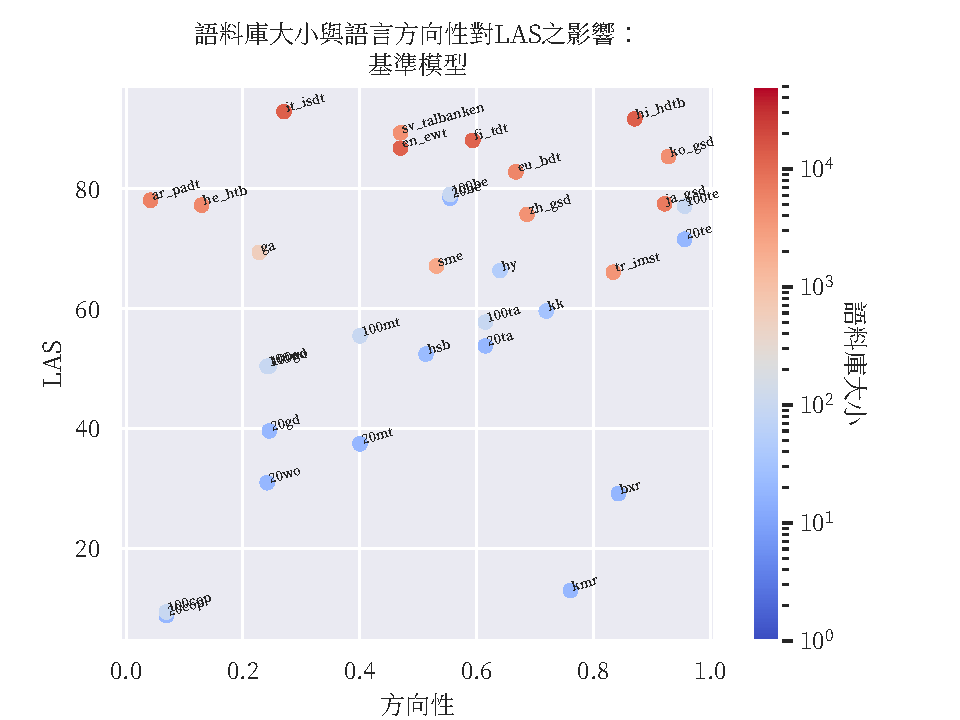
\includegraphics{figs/chapter3/dir_size_las_ft_multi.pdf}
    \caption{方向性與數據量對基準模型進行單語言\finetune後LAS的影響}
    \label{fig:dir-size-las-ft-multi}
\end{figure}

\begin{figure}[h]
    \centering
    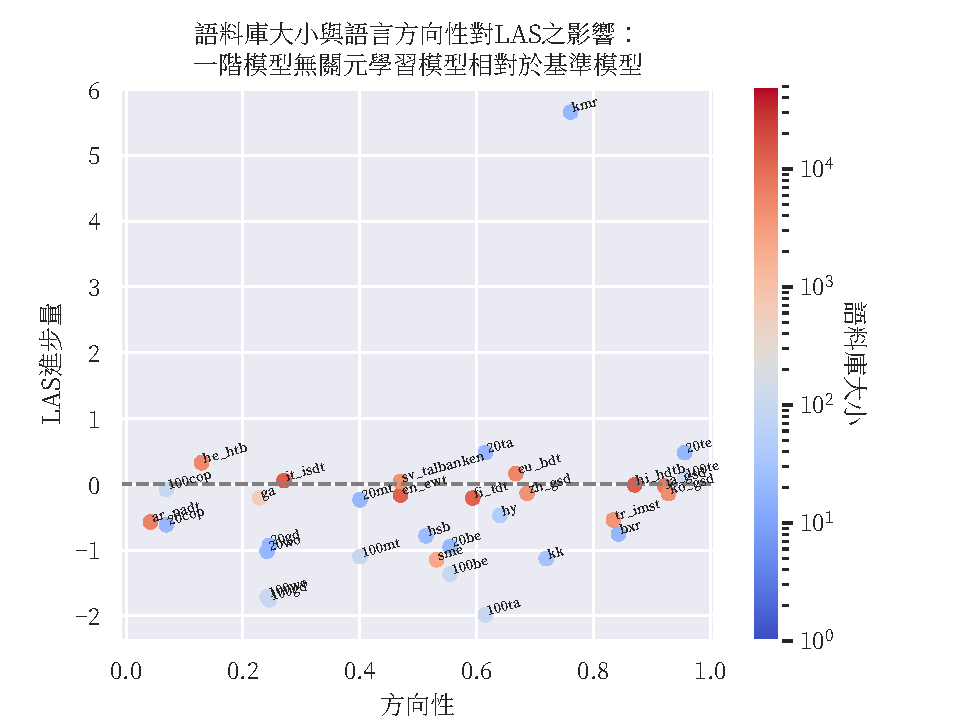
\includegraphics{figs/chapter3/dir_size_las_ft_fomaml-to-multi.pdf}
    \caption{方向性與句法樹庫大小對\fomaml 模型相對於基準模型各自進行單語言\finetune 後LAS之進步量的影響}
    \label{fig:dir-size-las-ft-fomaml-to-multi}
\end{figure}

\begin{figure}[h]
    \centering
    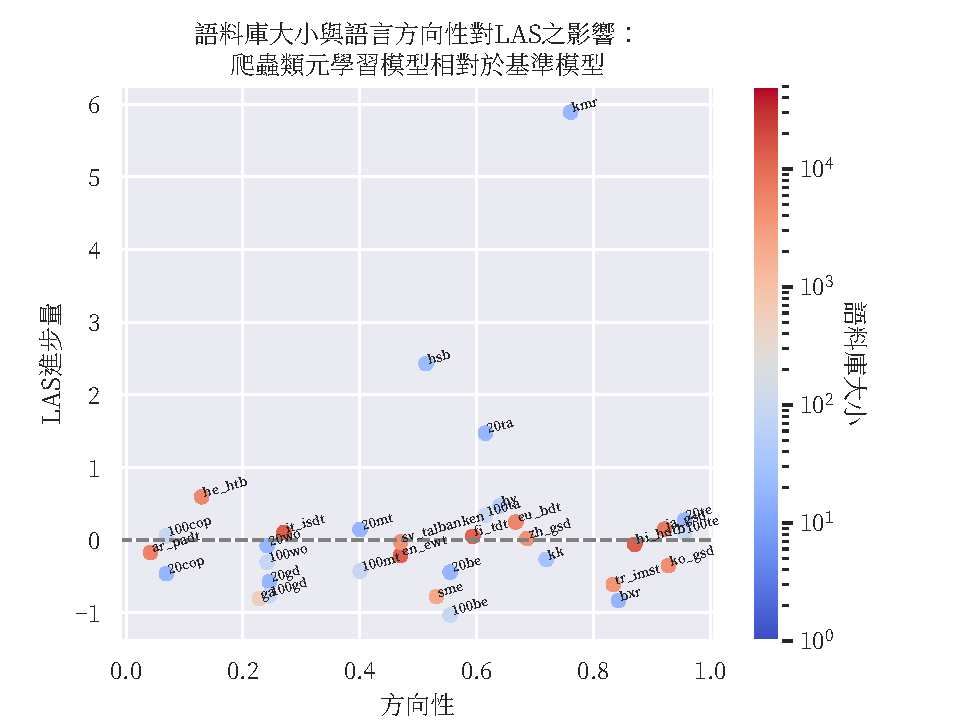
\includegraphics{figs/chapter3/dir_size_las_ft_reptile-to-multi.pdf}
    \caption{方向性與句法樹庫大小對\reptile 模型相對於基準模型各自進行單語言\finetune 後LAS之進步量的影響}
    \label{fig:dir-size-las-ft-reptile-to-multi}
\end{figure}

